% !TeX program = lualatex
\documentclass{article}
\usepackage[14pt]{extsizes}

% Begin embedded preamble-345.tex (edit packages and macros here).
\parindent 0em
\parskip0em
% Allow long mathematical terms to wrap without protruding into the margins.
\setlength{\emergencystretch}{2em}
\topmargin -2.0 truecm
\textheight 24 truecm
\textwidth 17.5 truecm
\oddsidemargin -1 truecm
\evensidemargin -1 truecm

% Times-style fonts for both pdfLaTeX and LuaLaTeX/XeLaTeX.
\usepackage{iftex}
\usepackage{amsmath}
\usepackage{enumerate}
\ifPDFTeX
  \usepackage[T1]{fontenc}
  \usepackage{tgtermes}
  \usepackage{newtxmath}
\else
  \usepackage{fontspec}
  \setmainfont{TeX Gyre Termes}
  \usepackage{unicode-math}
  \setmathfont{TeX Gyre Termes Math}
\fi
\usepackage{fancyhdr}
\usepackage{color}
\usepackage{graphicx}
\usepackage{pgf,tikz,pgfplots}
\pgfplotsset{compat=1.18}
\usetikzlibrary{arrows, shapes.geometric, matrix, turtle, plotmarks}
\usepackage{url}
\usepackage{xcolor}
\usepackage{dashrule}



%%%


\definecolor{answercolor}{RGB}{148,0,211}  % Purple color for answers
% Answer functionality
\newif\ifshowanswers
\showanswersfalse  % Default to hiding answers
% Command to show/hide answers
\newcommand{\printanswers}{\showanswerstrue}
\newcommand{\hideanswers}{\showanswersfalse}
% Answer Box Commands
% Usage:
%   \answer{math content}         - Creates box with default height (4cm)
%   \answer[6cm]{math content}    - Creates box with specified height
% The box height remains constant whether answers are shown or hidden
% (\printanswers or \hideanswers), ensuring consistent page layout.
\newcommand{\answer}[2][4cm]{%
	\noindent\framebox[\textwidth]{%
		\begin{minipage}[t][#1][t]{\dimexpr\textwidth-2\fboxsep-2\fboxrule\relax}
			\ifshowanswers
			{\color{answercolor}#2\par}
			\fi
		\end{minipage}%
	}
}
\newcommand\shortanswer[1]{%
	\ifshowanswers%
	\underline{\color{answercolor}{\hspace{0.5em} #1\hspace{0.5em}}}%
	\else%
	\underline{\phantom{\hspace{0.5em} #1\hspace{0.5em}}}%
	\fi%
}



\definecolor{fillincolor}{RGB}{148,0,211}  % Purple color for fillin-ins
% Fiil-in functionality
\newif\ifshowfillins
\showfillinsfalse  % Default to hiding answers
% Command to show/hide answers
\newcommand{\printfillins}{\showfillinstrue}
\newcommand{\hidefillins}{\showfillinsfalse}
\newcommand\fillin[1]{%
	\ifshowfillins%
	\underline{\color{fillincolor}{\hspace{0.5em} #1\hspace{0.5em}}}%
	\else%
	\underline{\phantom{\hspace{0.5em} #1\hspace{0.5em}}}%
	\fi%
}


%%%

\pagestyle{fancy}

\renewcommand{\headrulewidth}{0pt}
%\lhead{\tiny Math 345: Spring 2025, copyright: Lindsey, Zimmer, Roch}
\lhead{\tiny Math 345: Spring 2025, copyright: Phillipson, Roch}



\newcommand\displayspace[1]{\begin{multline*}
    \shoveright {#1}
    \end{multline*}}

\newcommand{\ruleone}{\rule{1in}{0.0005in}}
\newcommand{\ruleonepfive}{\rule{1.5in}{0.0005in}}
\newcommand{\ruletwo}{\rule{2in}{0.0005in}}

\newcommand{\hspaceone}{\hspace{1in}}

\newcommand{\bbR}{\mathbb{R}}

\newcommand{\calF}{{\mathcal{F}}}
\newcommand{\inv}{{^{-1}}}
\newcommand{\Ainv}{{A^{-1}}}
\newcommand{\by}{{\times}}

\DeclareMathOperator{\adj}{adj}
\DeclareMathOperator{\spn}{span}
\DeclareMathOperator{\rank}{rank}
\DeclareMathOperator{\nullity}{nullity}
\DeclareMathOperator{\Tr}{tr}
\DeclareMathOperator{\range}{range}
\DeclareMathOperator{\minor}{minor}
\DeclareMathOperator{\cof}{cof}
\DeclareMathOperator{\diag}{diag}
\DeclareMathOperator{\im}{im}
\DeclareMathOperator{\col}{col}
\DeclareMathOperator{\row}{row}
\DeclareMathOperator{\nool}{null}



\newcommand\ola[1]{\textcolor{magenta}{O: #1}}
\newcommand\peti[1]{\textcolor{teal}{P: #1}}
\newcommand\rub[1]{\textcolor{teal}{#1}}
\newcommand\points[1]{\textcolor{blue}{\textrm{+#1}}}

%%%%%%%%%%%%%%%%%%%
%%%headings etc.
%%%%%%%%%%%%%%%%%%%



\newcommand\notice{\textit{Notice:} }
\newcommand\question{\textbf{Question:} }
\newcommand\proof{\textbf{Why is it true?} }
\newcommand\setup{\textit{Set-up:} }
\newcommand\idea{\textit{Idea:} }
\newcommand\warning{\textbf{Warning:} }
\newcommand\topic[1]{\subsubsection*{#1}}
% The online notes embed the video; the PDF points readers to it.
\newcommand\video[2][]{\par\textit{A video tutorial for this section is in the online notes.}\par}


% Create a common counter for all theorem-like environments
\newcounter{commoncount}

% Redefine the commands to use the counter
\newcommand\activity{\refstepcounter{commoncount}\textbf{Activity \thecommoncount:} }
\newcommand\theorem{\refstepcounter{commoncount}\textbf{Theorem \thecommoncount:} }
\newcommand\corollary{\refstepcounter{commoncount}\textbf{Corollary \thecommoncount:} }
\newcommand\lemma{\refstepcounter{commoncount}\textbf{Lemma \thecommoncount:} }
\newcommand\fact{\refstepcounter{commoncount}\textbf{Fact \thecommoncount:} }
\newcommand\note{\refstepcounter{commoncount}\textbf{Note \thecommoncount:} }
\newcommand\definition{\refstepcounter{commoncount}\textbf{Definition \thecommoncount:} }
\newcommand\remark{\refstepcounter{commoncount}\textit{Remark \thecommoncount:} }

% Section headings and PDF bookmarks.
\newcommand\sectiontitle[2]{\subsection*{Section #1: #2}%
  \addcontentsline{toc}{subsection}{Section #1: #2}}
\newcommand\chaptertitle[2]{\section*{Chapter #1: #2}%
  \addcontentsline{toc}{section}{Chapter #1: #2}}

% Boxed lecture material with breakable text and horizontal rules.
\newenvironment{framed}{\par\medskip\hrule\smallskip}
  {\par\smallskip\hrule\medskip}

%matrix entries 
\newcommand{\aaa}[2]{{a_{#1#2}}}
\newcommand{\aij}{{a_{ij}}}
\newcommand{\bbb}[2]{{b_{#1#2}}}
\newcommand{\bij}{{b_{ij}}}
\newcommand{\ccc}[2]{{c_{#1#2}}}
\newcommand{\cij}{{c_{ij}}}

%matrix minors and cofactors 
\newcommand{\Aij}{{A_{ij}}}
\newcommand{\Mij}{{M_{ij}}}


%dimension shortcuts 
\newcommand{\mbyn}{{m \times n}}
\newcommand{\nbyn}{{n \times n}}

%vectors 
\newcommand{\veca}{{\vec{a}}}
\newcommand{\bmata}{{\left[ \begin{array}{r} a_1 \\ a_2 \\ \ldots \\ a_n \end{array} \right] }}
\newcommand{\bmatb}{{\left[ \begin{array}{r} b_1 \\ b_2 \\ \ldots \\ b_n \end{array} \right] }}
\newcommand{\bmatx}{{\left[ \begin{array}{r} x_1 \\ x_2 \\ \ldots \\ x_n \end{bmatrix}{r} \right]}}

\newcommand{\colvec}[1]{{\left[ \begin{array}{r} #1 \end{array} \right]}}
\newcommand{\ccolvec}[1]{{\left[ \begin{array}{c} #1 \end{array} \right]}}
\newcommand{\twovec}[2]{{\left[ \begin{array}{r} #1 \\ #2 \end{array} \right]}}
\newcommand{\threevec}[3]{{\left[ \begin{array}{r} #1 \\ #2 \\ #3 \end{array} \right]}}
\newcommand{\fourvec}[4]{{\left[ \begin{array}{r} #1 \\ #2 \\ #3 \\ #4 \end{array} \right]}}

\newcommand{\colvecb}{{\left[ \begin{array}{c} b_1 \\ b_2 \\ \vdots \\ b_n \end{array} \right]}}
\newcommand{\colvecbm}{{\left[ \begin{array}{c} b_1 \\ b_2 \\ \vdots \\ b_m \end{array} \right]}}
\newcommand{\colvecc}{{\left[ \begin{array}{c} c_1 \\ c_2 \\ \vdots \\ c_n \end{array} \right]}}
\newcommand{\colvecx}{{\left[ \begin{array}{c} x_1 \\ x_2 \\ \vdots \\ x_n \end{array} \right]}}

\newcommand{\threerowvec}[3]{{\left[ \begin{array}{rrr} #1 & #2 & #3 \end{array} \right]}}
\newcommand{\fourrowvec}[4]{{\left[ \begin{array}{rrr} #1 & #2 & #3 & #4 \end{array} \right]}}

%matrix commands 
\newcommand{\twobytwo}[4]{{\left[ \begin{array}{rr} #1 & #2 \\ #3 & #4 \end{array} \right]}}
\newcommand{\cIthree}[1]{{\left[ \begin{array}{rrr} #1 & 0 & 0 \\ 0 & #1 & 0 \\ 0 & 0 & #1 \end{array} \right]}}
\newcommand{\barray}[2]{{\left[ \begin{array}{#1} #2 \end{array} \right]}}
\newcommand{\Amn}{{\left[ \begin{array}{cccc} 
a_{11} & a_{12} & \cdots & a_{1n} \\ 
a_{21} & a_{22} & \cdots & a_{2n} \\ 
\vdots & \vdots & \ddots & \vdots \\ 
a_{m1} & a_{m2} & \cdots & a_{mn}
\end{array} \right]}}
\newcommand{\Ann}{{\left[ \begin{array}{cccc} 
a_{11} & a_{12} & \cdots & a_{1n} \\ 
a_{21} & a_{22} & \cdots & a_{2n} \\ 
\vdots & \vdots & \ddots & \vdots \\ 
a_{n1} & a_{n2} & \cdots & a_{nn}
\end{array} \right]}}
\newcommand{\Amnb}{{\left[ \begin{array}{cccc|c} 
a_{11} & a_{12} & \cdots & a_{1n} & b_1 \\ 
a_{21} & a_{22} & \cdots & a_{2n} & b_2 \\ 
\vdots & \vdots & & \vdots & \vdots \\ 
a_{m1} & a_{m2} & \cdots & a_{mn} & b_m
\end{array} \right]}}

%math boldface

\newcommand{\bfa}{{\mathbf{a}}}
\newcommand{\bfb}{{\mathbf{b}}}
\newcommand{\bfc}{{\mathbf{c}}}
\newcommand{\bfd}{{\mathbf{d}}}
\newcommand{\bfe}{{\mathbf{e}}}
\newcommand{\bff}{{\mathbf{f}}}
\newcommand{\bfi}{{\mathbf{i}}}
\newcommand{\bfj}{{\mathbf{j}}}
\newcommand{\bfk}{{\mathbf{k}}}
\newcommand{\bfu}{{\mathbf{u}}}
\newcommand{\bfv}{{\mathbf{v}}}
\newcommand{\bfw}{{\mathbf{w}}}
\newcommand{\bfx}{{\mathbf{x}}}
\newcommand{\bfy}{{\mathbf{y}}}
\newcommand{\bfz}{{\mathbf{z}}}
\newcommand{\bfzero}{{\mathbf{0}}}
\newcommand{\bfone}{{\mathbf{1}}}


%%%%%%%%%%%%%%%%%%%%
%%%DASH LINE COMMAND
%%%%%%%%%%%%%%%%%%%%

\makeatletter
\newcommand*\dashline{\mathrel{\vert}}
\makeatother

%%%%%%%%%%%%%%%%%%%%
%%%INTEGRAL
%%%%%%%%%%%%%%%%%%%%

\newcommand{\ddd}{\mathrm{d}}

%%%%%%%%%%%%%%%%%%%
%%%%  TIKZ %%%%%%%%
%%%%%%%%%%%%%%%%%%%

\newcommand{\coordsys}[4]{
\foreach \x in {#1,...,#3}
\draw[line width=.6pt,color=black!15,dashed] (\x,#2-.2) -- (\x,#4+.2);
\foreach \y in {#2,...,#4}
\draw[line width=.6pt,color=black!15,dashed] (#1-.2,\y) -- (#3+.2,\y);
\draw[->] (#1-.2,0) -- (#3+.2,0) node[right] {$x$};
\draw[->] (0,#2-.2) -- (0,#4+.2) node[above] {$y$};
\foreach \x in {#1,...,-1}
\draw[shift={(\x,0)},color=black] (0pt,2pt) -- (0pt,-2pt) node[below] {\footnotesize $\x$};
\foreach \x in {1,...,#3}
\draw[shift={(\x,0)},color=black] (0pt,2pt) -- (0pt,-2pt) node[below] {\footnotesize $\x$};
\foreach \y in {#2,...,-1}
\draw[shift={(0,\y)},color=black] (2pt,0pt) -- (-2pt,0pt) node[left] {\footnotesize $\y$};
\foreach \y in {1,...,#4}
\draw[shift={(0,\y)},color=black] (2pt,0pt) -- (-2pt,0pt) node[left] {\footnotesize $\y$};
}


%%%

% PDF links and document information
\usepackage{hyperref}
\hypersetup{
	pdftitle={Math 345 - Chapter 2: Matrix Algebra},
	pdfauthor={Sebastien Roch},
	pdfsubject={Linear algebra and optimization},
	pdfkeywords={linear algebra, lecture notes, mathematics},
	pdfstartview=Fit,
	pdfinfo={
		Title={Math 345 - Chapter 2: Matrix Algebra}
	}
}
% End embedded preamble-345.tex

% Commands to show/hide answers/fillins
% Uncomment if needed
% Default is hiding
\printanswers
\printfillins


\begin{document}


\chaptertitle{2}{Matrix Algebra}
{\small These notes use material from your textbook \textit{Linear Algebra with Applications} by W. Keith Nicholson [LAWA]. Sections are numbered in their order of presentation within each chapter.}

\bigskip

{\small
Learning goals:
\begin{itemize}
	\item Be able to pick out an element of a matrix given its indices
	\item Know what it means for two matrices to be equal vs. row equivalent
	\item Know how to perform matrix operations: sum/difference, scalar multiplication, transpose,
	matrix-vector product (both as a linear combination and using dot product)
	\item Know the basic properties of matrix operations
	\item Know how to perform matrix multiplication (both as repeated matrix-vector multiplication
	and using dot product)
	\item Know which sizes of matrices can be multiplied together, and what the resulting product
	matrix’s size will be
	\item Know the properties of matrix multiplication and how they interact with previous
	operations
	\item Be familiar with properties of inverses of matrices: uniqueness, inverse of a product,
	inverse of inverse, inverse of transpose
	\item Know how to use matrix inverses to solve linear systems of equations
	\item Be able to compute inverse matrices directly using row reduction
	\item Know the equivalent properties to determine if a matrix is invertible
	\item Know how to find the inverse of a matrix transformation
	\item Be able to compute the image of a vector under a matrix transformation
	\item Be able to determine if a vector is the image of vector under a matrix transformation
	\item Find the matrix representation of a linear transformation $T:\mathbb{R}^n\to \mathbb{R}^m$
	
\end{itemize}
}

%\bigskip	
\newpage


\sectiontitle{2.1}{Matrix Addition, Scalar Multiplication, and Transposition}


We've seen matrices used to help us solve systems of linear equations. We're now going to define them more formally and explore other ways to utilize them.

\definition An $m \times n$ \fillin{matrix} $A$ is a rectangular array of $m \cdot n$ real numbers arranged in $m$ \fillin{horizontal rows} and $n$ \fillin{vertical columns}: 
\[
A = \begin{bmatrix}
\aaa11 & \aaa12 & \cdots & \cdots & \cdots & \aaa1n \\ 
\aaa21 & \aaa22 & \cdots & \cdots & \cdots & \aaa2n \\ 
\vdots & \vdots & \cdots & \cdots & \cdots & \vdots \\ 
\vdots & \vdots & \cdots & \cdots & a_{ij} & \vdots \\ 
\vdots & \vdots & \cdots & \cdots & \cdots & \vdots \\ 
a_{m1} & a_{m2} & \cdots & \cdots & \cdots & a_{mn} \\ 
\end{bmatrix} 
\]
The \fillin{$i$th row} of $A$ is 
$\begin{bmatrix}
a_{i1} & a_{i2} & \cdots & a_{in}
\end{bmatrix},$ and the \fillin{$j$-th column} of $A$ is 
\[ 
\begin{bmatrix}
\aaa1j \\ \aaa2j \\ \vdots \\ a_{mj}.
\end{bmatrix}.
\]
The number $\aij$, which is in the $i$th row and $j$th column of $A$, is the \fillin{$(i,j)$-entry} of $A$, and we often write \(A = [\aij].\)  We say $A$ is an ``\fillin{$m$ by $n$}'' matrix.

\bigskip

\activity Consider the matrix 
\[
A = \begin{bmatrix}
1 & 2 & 3 \\ 
5 & -8 & -13
\end{bmatrix}
\]
$A$ is a \shortanswer{2} $\times$ \shortanswer{3} matrix. Complete the following:

\bigskip

\begin{minipage}{0.49\textwidth}
\begin{itemize}
    \item $\aaa11 = \shortanswer{1}$ 
    \item $\aaa12 = \shortanswer{2}$ 
    \item $\aaa21 = \shortanswer{5}$ 
\end{itemize}
\end{minipage}
\begin{minipage}{0.49\textwidth}
\begin{itemize}
    \item $\aaa23 = \shortanswer{-13}$ 
    \item $\aaa32 = \shortanswer{\text{no such entry}}$ 
\end{itemize}
\end{minipage}

\bigskip

\definition Two matrices $A$ and $B$ are \fillin{equal} if they have the same size AND all the corresponding entries are equal.

\newpage

\activity If $A=\begin{bmatrix} 3 & y\\ 4 & -7\end{bmatrix}$ and $B=\begin{bmatrix} 6+x & -2 \\4 & -7 \end{bmatrix}$, and $A=B$, find $x$ and $y$.

\bigskip

\answer[5cm]{Since $A = B$, comparing corresponding entries:
	\[ 3 = 6 + x \implies x = -3 \]
	\[ y = -2 \]
	Therefore $x = -3$ and $y = -2$.}
	
	\bigskip

\topic{Matrix Operations} 

\textit{Matrix Addition}: If $A = [\aij]$ and $B = [\bij]$ are both $m \times n$ matrices, then their \fillin{sum} $A+B$ is the matrix $C = [\cij]$ where $\cij =$ \fillin{$\aij + \bij$}.

\bigskip 

\activity For the matrices $A$ and $B$ as below, calculate $A+B$. 
\[
A = \begin{bmatrix}
1 & 2 & 3 \\ 
5 & -8 & -13
\end{bmatrix}
\quad
\text{and}
\quad 
B = \begin{bmatrix}
0 & 2 & 1 \\ 
1 & 3 & -4 
\end{bmatrix}
\]

\answer[2cm]{
	$$
	A+B = \begin{bmatrix} 1 & 4 & 4\\ 6 & -5 & -17\end{bmatrix}
	$$}
\bigskip

\note For $A+B$ to be defined, $A$ and $B$ must be the same size. From now on, if we write $A+B$, assume that this is the case. 

\bigskip 

\textit{Scalar Multiplication}: If $A = [\aij]$ is an $\mbyn$ matrix and $r$ is a real number, then the \fillin{scalar multiple} of $A$ by $r$, written \fillin{$rA$}, is the $\mbyn$ matrix $C = [\cij]$, where $\cij = $\fillin{$r\aij$}, that is, $C$ is the matrix obtained by multiplying every entry of $A$ by $r$. 

\bigskip 

\activity For $A$ as in the activity above, calculate $-2A$. 

\answer[2cm]{\[-2A = \begin{bmatrix} -2 & -4 & -6 \\ -10 & 16 & 26 \end{bmatrix}\]}

\bigskip


\definition If $A_1, A_2, \ldots, A_k$ are $\mbyn$ matrices and $c_1, c_2, \ldots, c_k$ are real numbers, then an expression of the form 
\[
c_1 A_1 + c_2 A_2 + \cdots + c_k A_k
\]
is called a \fillin{linear combination} of $A_1, A_2, \ldots, A_k$. The scalars $c_1, \ldots, c_k$ are called \fillin{coefficients}. 

\bigskip

\activity The following is a linear combination of matrices. Compute it. 

\bigskip

$
4 \begin{bmatrix} 
0 & 2  \\ 
-3 & 3  
\end{bmatrix}
- \frac{1}{2} \begin{bmatrix}
4 & 2  \\
6 & 2  
\end{bmatrix}
$

\bigskip

\answer[5cm]{\begin{align*}
		&= \begin{bmatrix} 0 & 8 \\ -12 & 12 \end{bmatrix} - \begin{bmatrix} 2 & 1 \\ 3 & 1 \end{bmatrix} \\
		&= \begin{bmatrix} -2 & 7 \\ -15 & 11 \end{bmatrix}
\end{align*}}

\bigskip



\topic{Matrix Addition Properties}
Let $A$, $B$, and $C$ be $\mbyn$ matrices. 
\begin{enumerate}[(a)]
    \item $A+B = $ \fillin{$A + B$}, i.e. matrix addition is \fillin{commutative}.
    \item $A + (B + C) =$ \fillin{$(A + B) + C$}, i.e. matrix addition is \fillin{associative}.
    \item There is a unique $\mbyn$ matrix $O$ such that $A+O = $\fillin{$A$} for any $\mbyn$ matrix $A$. The matrix $O$ is called the $\mbyn$ \fillin{zero matrix}.  
    \item For each $\mbyn$ matrix $A$, there is a unique $\mbyn$ matrix $D$ such that $A+D=$\fillin{$O$}. The matrix $D$ must, in fact, be the matrix \fillin{$- A = (-1)A$}. The matrix $-A$ is called the \fillin{negative} of $A$.
\end{enumerate}

\textit{Proof of (a) (if time)}: 


\answer{Let $A = [a_{ij}]$ and $B = [b_{ij}]$. Then:
	\begin{align*}
		A + B &= [a_{ij} + b_{ij}] \\
		&= [b_{ij} + a_{ij}] \quad \text{(since real numbers are commutative)} \\
		&= B + A
	\end{align*}
}
	

%\bigskip
\newpage

\topic{Scalar Multiplication Properties} If $r$ and $s$ are real numbers and $A$ and $B$ are matrices of the appropriate sizes, then 
\begin{enumerate}[(a)]
    \item $r(sA)=$\fillin{$(rs) A$}.
    \item $(r+s)A=$\fillin{$rA + sA$}. 
    \item $r(A+B)=$\fillin{$rA + rB$}. 
\end{enumerate}


\definition If $A = [\aij]$ is an $\mbyn$ matrix, then the \fillin{transpose} of $A$, denoted \\$A^T = [\aij^T]$, is the \fillin{$n$} $\times$ \fillin{$m$} matrix defined by 
$$\aij^T = a_{ji}$$ 
In other words, the transpose of $A$ is obtained by \fillin{interchanging} the rows and the columns of $A$.

\bigskip 

\activity Compute the transpose for each of the given matrices: 
\[
A = 
\begin{bmatrix}
1 & 2 & 3 \\ 
5 & -8 & -13
\end{bmatrix}, 
\ \ 
B = 
\begin{bmatrix}
5 & 2 & 3 \\
6 & 2 & 3 \\ 
-1 & -2 & 3
\end{bmatrix}, 
\text{ and } 
C = 
\begin{bmatrix}
10 \\ 20 \\ 30 
\end{bmatrix}.
\]

\bigskip

\answer[7cm]{
	$A^T = \begin{bmatrix} 1 & 5 \\ 2 & -8 \\ 3 & -13 \end{bmatrix}$
	
	$B^T = \begin{bmatrix} 5 & 6 & -1 \\ 2 & 2 & -2 \\ 3 & 3 & 3 \end{bmatrix}$
	
	$C^T = \begin{bmatrix} 10 & 20 & 30 \end{bmatrix}$}
	
%\bigskip
\newpage

\definition
If $A=[a_{ij}]$ is an $m\times n$ matrix, the elements
$a_{11}, a_{22}, a_{33},\ldots $ are called the main diagonal of $A$. 
\begin{figure}[!h]
	\centering
	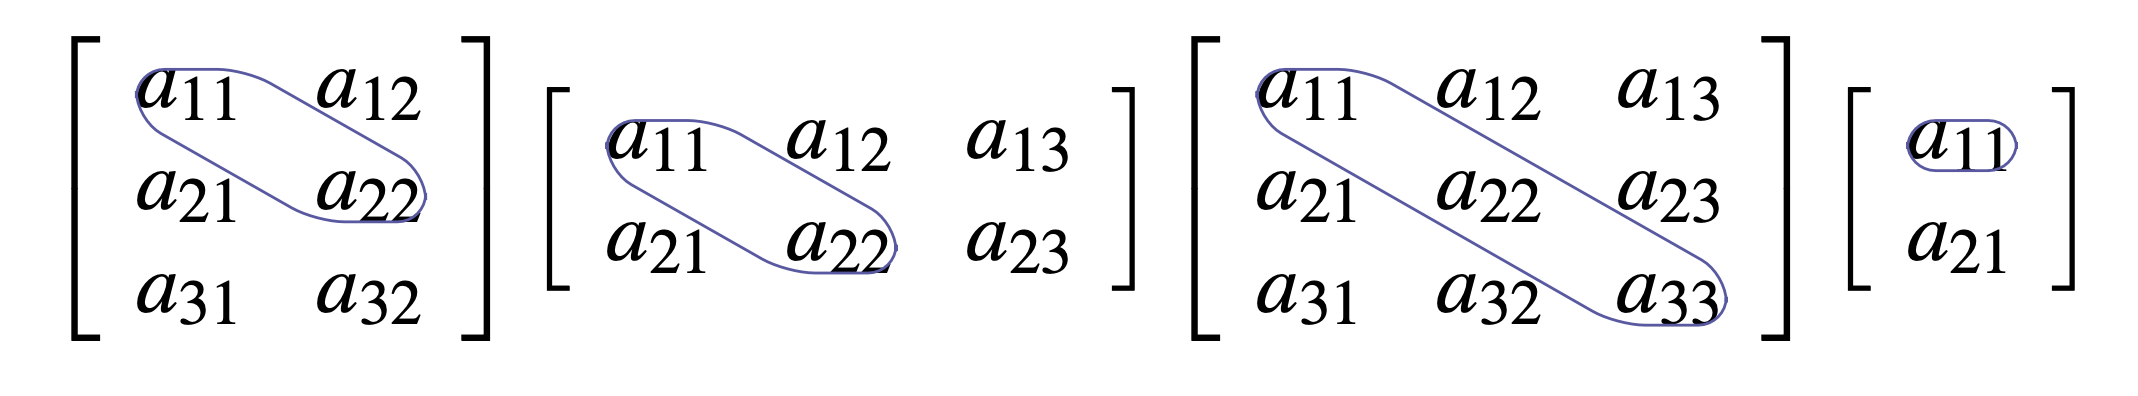
\includegraphics[width=6in]{diagonal}
	\caption{From Linear Algebra with Applications, Vretta-Lyryx}
\end{figure}

\bigskip


Thus forming the transpose of a matrix $A$ can be viewed as \fillin{flipping} $A$ about its main diagonal. 


\bigskip

\topic{Matrix Transpose Properties} 
If $r$ is a scalar and $A$ and $B$ are matrices of the appropriate sizes, then 
\begin{enumerate}[(a)]
    \item $(A^T)^T =$\fillin{$A$}
    \item $(A + B)^T=$\fillin{$A^T + B^T$}
    \item $(rA)^T=$\fillin{$rA^T$}
\end{enumerate}

\textit{Proof of (b) (time permitting):}

\answer[6cm]{Let $A = [a_{ij}]$ and $B = [b_{ij}]$. Then $A + B = [c_{ij}]$ where $c_{ij} = a_{ij} + b_{ij}$.
	
	By definition of transpose: $(A + B)^T = [c_{ij}]^T = [c_{ji}]$
	
	Since $c_{ij} = a_{ij} + b_{ij}$, we have:
	$[c_{ji}] = [a_{ji} + b_{ji}] = [a_{ji}] + [b_{ji}] = A^T + B^T$
	
	Therefore, $(A + B)^T = A^T + B^T$.}
	
		
\bigskip

\definition A matrix $A$ with real entries is called \fillin{symmetric} if \fillin{$A^T = A$}. A matrix $A$ is called \fillin{skew symmetric} if \fillin{$A^T = -A$}. 

%\bigskip 
\newpage

\activity Are the following matrices symmetric/skew symmetric/neither? 
\begin{itemize}
    \item[] $A = \barray{rrr}{0 & 2 & -3 \\ -2 & 0 & 5 \\ 3 & -5 & 0}, \quad B = \barray{rrr}{3 & 5 & 2 \\ 5 & 1 & 4 \\ 2 & 4 & -1},$
    \item[] $C = \barray{rrr}{1 & 2 & -3 \\ -2 & 0 & 5 \\ 3 & 5 & 0}, \quad D = \barray{rrr}{0 & 0 & 0 \\ 0 & 0 & 0 \\ 0 & 0 & 0}.$
\end{itemize}

\answer[14cm]{Let's examine each matrix:
	\begin{enumerate}[(a)]
		\item $A = \begin{bmatrix} 0 & 2 & -3 \\ -2 & 0 & 5 \\ 3 & -5 & 0 \end{bmatrix}$
		skew symmetric since $A^T = -A$
		
		\item $B = \begin{bmatrix} 3 & 5 & 2 \\ 5 & 1 & 4 \\ 2 & 4 & -1 \end{bmatrix}$
		symmetric since $B^T = B$
		
		\item $C = \begin{bmatrix} 1 & 2 & -3 \\ -2 & 0 & 5 \\ 3 & 5 & 0 \end{bmatrix}$
		neither symmetric nor skew symmetric
		
		\item $D = \begin{bmatrix} 0 & 0 & 0 \\ 0 & 0 & 0 \\ 0 & 0 & 0 \end{bmatrix}$
		both symmetric and skew symmetric
\end{enumerate}}

\note If a matrix $A$ is symmetric AND skew symmetric at the same time, then $A$ must be a \fillin{zero} matrix! (Why?)


\newpage


\sectiontitle{2.2}{Matrix-Vector Multiplication}

\topic{Vectors as matrices}

\definition
A matrix is a \fillin{row vector} if it is $1 \times n$ and is a\\ \fillin{column vector} if it is $n \times 1$. Often we will call them just \fillin{$n$-vectors} or ``vectors of length $n$'' denoted with bold-face font. For example, $\mathbf{x}$ or $\mathbf{v}$. $\mathbb{R}^n$ denotes the set of all $n$-vectors.

\bigskip

\activity $\mathbf{v}=\begin{bmatrix}  -3 \\ \sqrt{2} \\ 0\end{bmatrix}$ is a \shortanswer{3-vector}, or a vector in \shortanswer{$\mathbb{R}^3$}.

\bigskip

The \fillin{zero vector} in $\mathbb{R}^n$, denoted $\mathbf{0}$ or \fillin{$\vec{0}$}, is the $n$-vector consisting of all zeros.

\bigskip

An $m\times n$ matrix can be thought of a row of $n$ column vectors of length $m$:

$A=\begin{bmatrix}\mathbf{a}_1 & \mathbf{a}_2 &\cdots & \mathbf{a}_n\end{bmatrix}$, where $\mathbf{a}_i$ is the \fillin{$i$-th column} of $A$.

\bigskip


\topic{Matrix-Vector Product} 
We start with an activity.

\bigskip

\activity Consider the linear system
\[ 
\begin{array}{rrrrrrr}
    x & + & 2y & + & 3z & = & 6  \\
    2x & - & 3y & + & 2z & = & 14 \\ 
    3x & + & y & - & z & = &-2.
\end{array}
\]
Rewrite this system using a linear combination. 

\answer{\[x \begin{bmatrix} 1 \\ 2 \\ 3 \end{bmatrix} + y \begin{bmatrix} 2 \\ -3 \\ 1 \end{bmatrix} + z \begin{bmatrix} 3 \\ 2 \\ -1 \end{bmatrix} = \begin{bmatrix} 6 \\ 14 \\ -2 \end{bmatrix}\]}

\bigskip

\definition Let $A=\begin{bmatrix}\mathbf{a}_1 & \mathbf{a}_2 &\cdots & \mathbf{a}_n\end{bmatrix}$ be an $m\times n$ matrix, written in terms of its columns $\mathbf{a}_1, \mathbf{a}_2, \ldots, \mathbf{a}_n.$ If $\mathbf{x}=\begin{bmatrix} x_1 \\ x_2 \\ \vdots \\ x_n\end{bmatrix}$ is any $n$-vector, the \fillin{matrix-vector product} $A\mathbf{x}$ is defined to be
the $m$-vector given by:

$$A\mathbf{x}=x_1\mathbf{a}_1+x_2\mathbf{a}_2+\cdots x_n\mathbf{a}_n.$$
 

\activity Compute the matrix-vector product $A\bfx$ where
\[
A = \barray{rrr}{
-1 & 4 & -5 \\ 
3 & 1 & -2
}
\text{ and } 
\bfx = \colvec{2 \\ -3 \\ 4}.
\]
%\answer[7cm]{
%	\begin{align*}&A\bfx =
%	\begin{bmatrix} -1 & 4 & -5 \\ 3 & 1 & -2 \end{bmatrix}
%	\begin{bmatrix} 2 \\ -3 \\ 4 \end{bmatrix}\\ 
%	&=
%	\begin{bmatrix} (-1)(2) + (4)(-3) + (-5)(4) \\ (3)(2) + (1)(-3) + (-2)(4) \end{bmatrix}\\
%	&=
%	\begin{bmatrix} -2 - 12 - 20 \\ 6 - 3 - 8 \end{bmatrix}
%	=
%	\begin{bmatrix} -34 \\ -5 \end{bmatrix}\end{align*}
%}
\answer[9cm]{
	\[A = \begin{bmatrix}\mathbf{a}_1 & \mathbf{a}_2 & \mathbf{a}_3\end{bmatrix} 
	\text{ where }
	\mathbf{a}_1 = \colvec{-1 \\ 3}, 
	\mathbf{a}_2 = \colvec{4 \\ 1}, 
	\mathbf{a}_3 = \colvec{-5 \\ -2}\]
	\begin{align*}
		A\bfx &= 2\mathbf{a}_1 + (-3)\mathbf{a}_2 + 4\mathbf{a}_3 \\[1ex]
		&= 2\colvec{-1 \\ 3} + (-3)\colvec{4 \\ 1} + 4\colvec{-5 \\ -2} \\[1ex]
		&= \colvec{-2 \\ 6} + \colvec{-12 \\ -3} + \colvec{-20 \\ -8} 
		= \colvec{-34 \\ -5}
	\end{align*}
}
%\bigskip


Notice that we can now write a linear system of equations in terms of a single matrix equation: 
Consider the linear system of $m$ equations in $n$ unknowns, 
\[
\begin{array}{llllll}
	a_{11}x_1 + & a_{12}x_2 + & \cdots + & a_{1n}x_n & = & b_1 \\
	a_{21}x_1 + & a_{21}x_2 + & \cdots + & a_{2n}x_n & = & b_2 \\ 
	\vdots & \vdots & & \vdots & & \vdots \\ 
	a_{m1}x_1 + & a_{m2}x_2 + & \cdots + & a_{mn}x_n & = & b_m.
\end{array}
\]
From this system, define the matrices
\[A = \Amn,
\quad
\bfx = \colvecx,
\text{ and } 
\bfb = \colvecbm.
\]

We can rewrite this system as a matrix equation: \shortanswer{$A\mathbf{x}=\mathbf{b}$}

%\bigskip
\newpage

\theorem 
\begin{enumerate}
    \item Every system of linear equations has the form $A\mathbf{x}=\mathbf{b}$ where $A$ is the coefficient matrix, $\mathbf{b}$ is
the constant matrix/vector, and $\mathbf{x}$ is the matrix/vector of variables.
\item The system $A\mathbf{x} =\mathbf{b}$ is consistent if and only if $\mathbf{b}$ is a linear combination of the columns of $A$.
\end{enumerate}

\activity Is $\mathbf{b}=\begin{bmatrix} 1 \\ 2 \\ 4\end{bmatrix}$ a linear combination of $\mathbf{a}_1=\begin{bmatrix} 1 \\3 \\-2\end{bmatrix}, \mathbf{a}_2=\begin{bmatrix} -2 \\1 \\1\end{bmatrix}$, $\mathbf{a}_3=\begin{bmatrix} -3 \\5 \\0\end{bmatrix}$?

\answer[18cm]{
	We need to solve the system:
	\[
	x_1 \begin{bmatrix} 1 \\ 3 \\ -2 \end{bmatrix} + x_2 \begin{bmatrix} -2 \\ 1 \\ 1 \end{bmatrix} + x_3 \begin{bmatrix} -3 \\ 5 \\ 0 \end{bmatrix} = \begin{bmatrix} 1 \\ 2 \\ 4 \end{bmatrix}
	\]
	which corresponds to the augmented matrix:
	
	\[
	\left[
	\begin{array}{rrr|r}
		1 & -2 & -3 & 1 \\
		3 & 1 & 5 & 2 \\
		-2 & 1 & 0 & 4
	\end{array}
	\right]
	\]
	
	$R_2 \to R_2 - 3R_1, \quad R_3 \to R_3 + 2R_1$:
	$
	\left[\begin{array}{rrr|r}
		1 & -2 & -3 & 1 \\
		0 & 7 & 14 & -1 \\
		0 & -3 & -6 & 6
	\end{array}\right]
	$
	
	$
	R_2 \to \frac{1}{7} R_2
	$:
	$
	\left[\begin{array}{rrr|r}
		1 & -2 & -3 & 1 \\
		0 & 1 & 2 & -\frac{1}{7} \\
		0 & -3 & -6 & 6
	\end{array}\right]
	$
	
	$
	R_3 \to R_3 + 3R_2
	$:
	$
	\left[\begin{array}{rrr|r}
		1 & -2 & -3 & 1 \\
		0 & 1 & 2 & -\frac{1}{7} \\
		0 & 0 & 0 & \frac{39}{7}
	\end{array}\right]
	$
	
	By the last row, the system is inconsistent, so no solution exists. Thus, \(\mathbf{b}\) is \textbf{not} a linear combination of the given vectors.
}


\bigskip

\activity If $\mathbf{x}=\mathbf{0}$, what is $A\mathbf{x}$? \shortanswer{$\mathbf{0}$}

If $A$ is the zero matrix, what is $A\mathbf{x}$? \shortanswer{$\mathbf{0}$}

\bigskip

\topic{Matrix-Vector Product Properties} Let $A$ and $B$ be $m\times n$ matrices, and let $\mathbf{x}$ and $\mathbf{y}$ be $n$-vectors in $\mathbb{R}^n$. Then:
\begin{itemize}
\item[a.] $A(\bfx+\bfy)=A\bfx+A\bfy$.
\item[b.] $A(r\bfx)=r(A\bfx)=(rA)\bfx$ for all scalars $r$.
\item[c.] $(A+B)\bfx=A\bfx+B\bfx$.
\end{itemize}

\textit{Proof of (b) (time permitting):}

\answer[17cm]{
	By the definition of matrix-vector multiplication, if \( A \) has columns \( \mathbf{a}_1, \mathbf{a}_2, \dots, \mathbf{a}_n \), then:
	$
	A\mathbf{x} = x_1 \mathbf{a}_1 + x_2 \mathbf{a}_2 + \dots + x_n \mathbf{a}_n.
	$
	
	Multiplying \( \mathbf{x} \) by \( r \) gives:
	$
	r\mathbf{x} = \begin{bmatrix} r x_1 \\ r x_2 \\ \vdots \\ r x_n \end{bmatrix}.
	$
	
	Applying \( A \) to this vector:
	
	\[
	A(r\mathbf{x}) = (r x_1) \mathbf{a}_1 + (r x_2) \mathbf{a}_2 + \dots + (r x_n) \mathbf{a}_n.
	\]
	%Factor out \( r \):
	\[
	A(r\mathbf{x}) = r (x_1 \mathbf{a}_1 + x_2 \mathbf{a}_2 + \dots + x_n \mathbf{a}_n) = r(A\mathbf{x}).
	\]
	
	If we multiply each column \( \mathbf{a}_j \) of \( A \) by \( r \), we get:
	
	\[
	rA = \begin{bmatrix} r\mathbf{a}_1 & r\mathbf{a}_2 & \dots & r\mathbf{a}_n \end{bmatrix}.
	\]
	
	Applying this to \( \mathbf{x} \):
	
	\[
	(rA)\mathbf{x} = x_1 (r\mathbf{a}_1) + x_2 (r\mathbf{a}_2) + \dots + x_n (r\mathbf{a}_n).
	\]
	%Factor out \( r \):
	\[
	(rA)\mathbf{x} = r(x_1 \mathbf{a}_1 + x_2 \mathbf{a}_2 + \dots + x_n \mathbf{a}_n) = r(A\mathbf{x}).
	\]
}

%\bigskip
\newpage

\topic{The Dot Product in $\mathbb{R}^n$}
We can express Matrix-Vector multiplication using dot products.

\bigskip

\definition An ordered sequence $(a_1, a_2, . . . , a_n)$ of real numbers is called an\\ 
\fillin{ordered $n$-tuple}.

\bigskip

\activity $(-2, \pi, 0, \dfrac{3}{4})$ is an ordered \fillin{four}-tuple.

\bigskip

\definition If $(a_1, a_2, . . . , a_n)$ and $(b_1, b_2, . . . , b_n)$ are two ordered $n$-tuples, their \\ 
\fillin{dot product} is defined to be the number 

$$a_1b_1+a_2b_2+\cdots a_nb_n$$

obtained by multiplying corresponding entries and adding the results.


\bigskip

\activity The dot product of $(-2, \pi, 0, \dfrac{3}{4})$ and $(3, 7, -4, 12)$ is

\answer{
	\begin{align*}
	&(-2)(3) + (\pi)(7) + (0)(-4) + \left(\frac{3}{4}\right)(12)\\ 
	&=
	-6 + 7\pi + 0 + 9 = 7\pi + 3.
	\end{align*}
}

\bigskip

\theorem Let $A$ be an $m\times n$ matrix and let $\mathbf{x}$ be an $n$-vector. Then each entry of the vector $A\mathbf{x}$ is the dot product of the corresponding row of $A$ with $\bfx$.
\begin{figure}[!h]
	\centering
	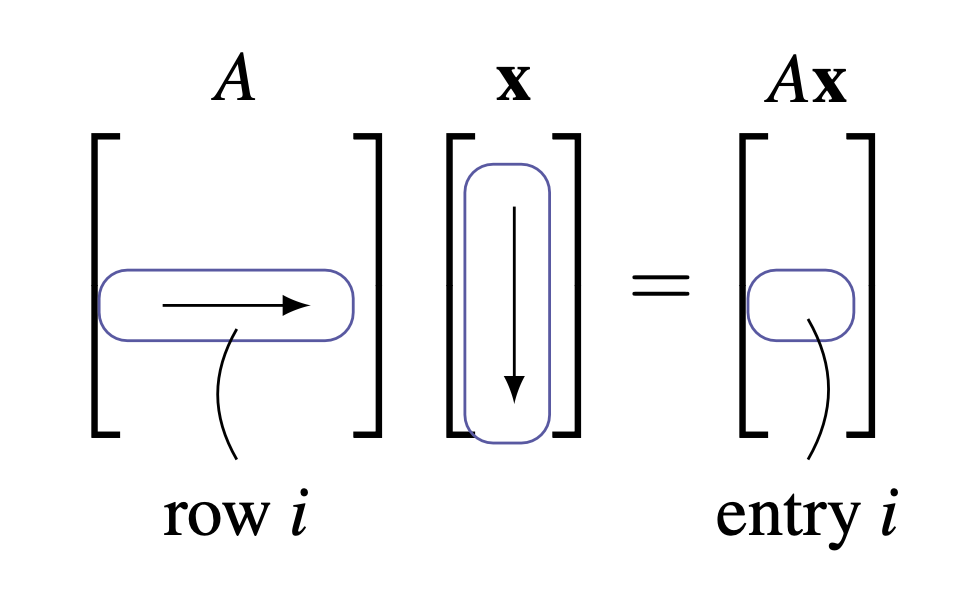
\includegraphics[width=3in]{Ax-dotproduct}
	\caption{From Linear Algebra with Applications, Vretta-Lyryx}
\end{figure}


%\medskip
%
%\begin{framed}
%Why do we have two definitions for matrix-vector product?
%
%\vspace{0.5in}
%\end{framed}

\newpage

\activity Compute the product $A\bfx$ using the dot product, where
\[
A = \barray{rrr}{
-1 & 4 & -5 \\ 
3 & 1 & -2
}
\text{ and } 
\bfx = \colvec{2 \\ -3 \\ 4}
\] 

\bigskip

\answer[6cm]{
	\begin{align*}
	&A\bfx =
	\begin{bmatrix} -1 & 4 & -5 \\ 3 & 1 & -2 \end{bmatrix}
	\begin{bmatrix} 2 \\ -3 \\ 4 \end{bmatrix}\\ 
	&=
	\begin{bmatrix} (-1)(2) + (4)(-3) + (-5)(4) \\ (3)(2) + (1)(-3) + (-2)(4) \end{bmatrix}
	=
	\begin{bmatrix} -34 \\ -5 \end{bmatrix}
	\end{align*}
}

\bigskip

\definition For each $n \geq 2$, the \fillin{identity matrix} $I_n$ is the $n\times n$ matrix with 1s on the main diagonal (upper left to lower right), and zeros elsewhere.

\begin{figure}[!h]
	\centering
	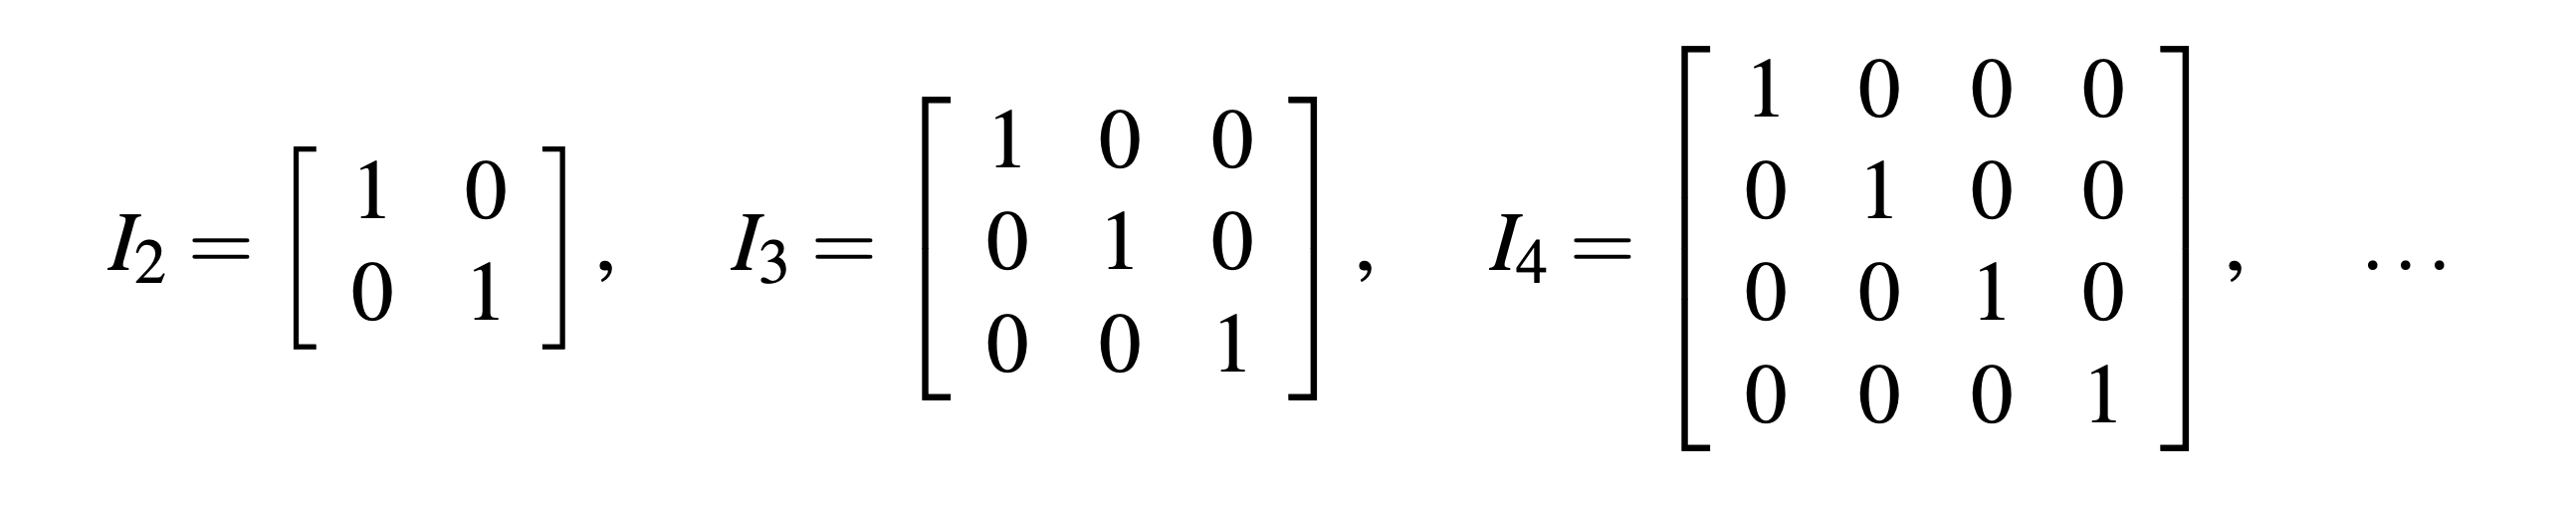
\includegraphics[width=6in]{identity}
	\caption{From Linear Algebra with Applications, Vretta-Lyryx}
\end{figure}




\fact For each $n\geq 2$ we have $I_n\bfx=\bfx$ for each $n$-vector $\bfx$ in $\mathbb{R}^n$.

\medskip

\activity Let's verify this fact for $I_3$.

\answer{
	\begin{align*}
	I_3 \bfx = \begin{bmatrix} 1 & 0 & 0 \\ 0 & 1 & 0 \\ 0 & 0 & 1 \end{bmatrix} 
	\begin{bmatrix} x_1 \\ x_2 \\ x_3 \end{bmatrix} = 
	\begin{bmatrix} x_1 \\ x_2 \\ x_3 \end{bmatrix} = \bfx.
	\end{align*}
}

%\bigskip
\newpage

\definition Consider $\mathbb{R}^n$, and let $\mathbf{e}_j$ denote the $j$th column of $I_n$, i.e, 


$$\mathbf{e}_j= \shortanswer{
	\begin{bmatrix}
		t_1 \\
		t_2 \\
		\vdots \\
		t_n
	\end{bmatrix}
	\text{ where } t_j = 1, \text{ but } t_i = 0 \text{ for all } i \neq j.}$$


These vectors are called the \fillin{standard basis vectors} for $\mathbb{R}^n$ (this name will make sense later).

\bigskip

\activity For $\mathbb{R}^4$, $\mathbf{e}_3$ is

\answer{
	\[
	\mathbf{e}_3 = \begin{bmatrix} 0 \\ 0 \\ 1 \\ 0 \end{bmatrix}.\]
}

\bigskip

Compute $A\mathbf{e}_3$ for $A=
\left[\begin{array}{cccc}
2 & 0 & 1 & -1 
\\
 3 & -1 & 4 & 0 
\\
 2 & -2 & 3 & -1 
\end{array}\right]
$

\bigskip

\answer{
	\[
	A\mathbf{e}_3 =
	\begin{bmatrix} 2 & 0 & 1 & -1 \\ 3 & -1 & 4 & 0 \\ 2 & -2 & 3 & -1 \end{bmatrix}
	\begin{bmatrix} 0 \\ 0 \\ 1 \\ 0 \end{bmatrix} =
	\begin{bmatrix} 1 \\ 4 \\ 3 \end{bmatrix}.\]
}


\bigskip

\fact If $A=\begin{bmatrix}\mathbf{a}_1 & \mathbf{a}_2 &\cdots & \mathbf{a}_n\end{bmatrix}$ be an $m\times n$ matrix, then $A\mathbf{e}_j=\mathbf{a}_j$ for $j=1\ldots n$.

\theorem Let $A$ and $B$ be $m\times n$ matrices. If $A\bfx=B\bfx$ for all $\bfx$ in $\mathbb{R}^n,$ then $A=B.$

\emph{Proof:}

\answer[3cm]{
	Since $A\bfx = B\bfx$ for all $\bfx$, choose $\bfx = \mathbf{e}_j$ for $j=1,\dots,n$. Then $A\mathbf{e}_j = B\mathbf{e}_j$ for all $j$. That is all the columns are the same, so $A=B$.
}

\bigskip

\topic{Transformations}

Geometric manipulations can be described via matrix-vector products.


\medskip 

Recall that we can interpret 2-vectors geometrically: $\begin{bmatrix} a_1 \\ a_2\end{bmatrix}$ corresponds to the point $(a_1,a_2)$ in the plane. To enhance this geometric representation of a vector $\begin{bmatrix} a_1 \\ a_2\end{bmatrix}$,  it is denoted graphically by an arrow from the origin $(0,0)$ to the point $(a_1,a_2)$. 

Similarly, we can define 3-vectors in space. 


\begin{minipage}{.45\textwidth}
\begin{center}
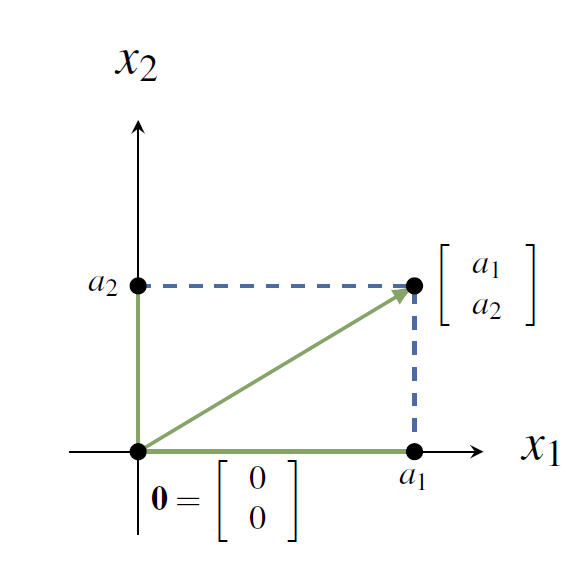
\includegraphics[scale=.85]{geom2vector.png}
\end{center}
\end{minipage}
\begin{minipage}{.45\textwidth}
    \begin{center}
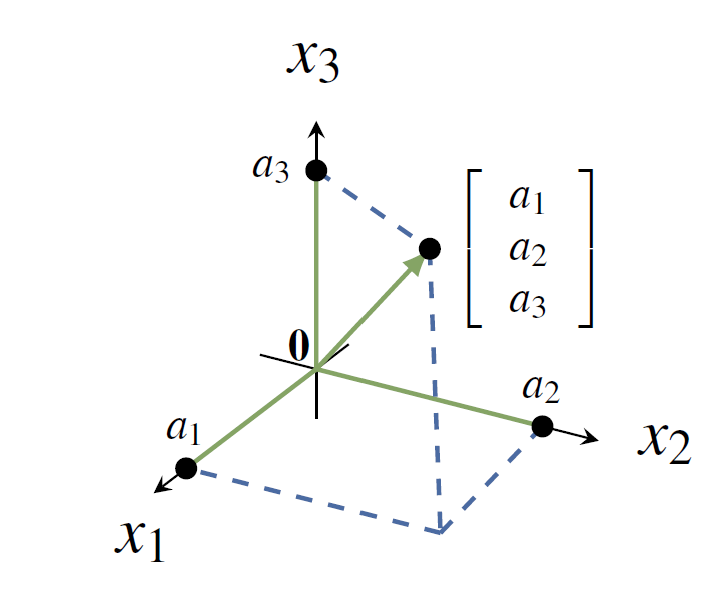
\includegraphics[scale=.8]{geom3vector.png}
\end{center}
\end{minipage}

%\activity Draw the geometric representation of 
%\[
%\bfv_1 = \colvec{2 \\ 2}, 
%\; 
%\bfv_2 = \colvec{1 \\ 0},
%\text{ and }
%\bfv_3 = \colvec{-3 \\ 1}.
%\]
%
%\vspace{1in} 

\activity Consider the transformation in $\mathbb{R}^2$ given by reflection across the $y$-axis, i.e.  $\begin{bmatrix} a_1 \\ a_2\end{bmatrix}$ gets sent to $ \begin{bmatrix} -a_1 \\ a_2\end{bmatrix}$. We can represent this reflection via a matrix-vector product: 

\bigskip

\answer[2cm]{
	\[A = \begin{bmatrix} -1 & 0 \\ 0 & 1 \end{bmatrix}\]
}

\bigskip

\definition Functions $T: \bbR^n \rightarrow \bbR^m$ are called \fillin{transformations} from $\mathbb{R}^n$ to $\mathbb{R}^m$. A transformation $T$ assigns a vector $\mathbf{x}$ in $\mathbb{R}^n$ a uniquely determined vector $T(\mathbf{x})$ in $\mathbb{R}^m$, called the \fillin{image} of $\bfx$ under $T$.

%\medskip
\newpage


\activity $T:\mathbb{R}^3\to\mathbb{R}^2$ given by 

$T\left(\begin{bmatrix} x_1 \\ x_2 \\ x_3\end{bmatrix}\right)=\begin{bmatrix} x_1 +x_3\\ x_2 \end{bmatrix}$ is a transformation.

What's the image of $\begin{bmatrix} 3 \\ -2 \\4\end{bmatrix}$ under $T$?


\answer[3cm]{
	\[T\left(\begin{bmatrix} 3 \\ -2 \\ 4\end{bmatrix}\right)
	= \begin{bmatrix} 3 + 4 \\ -2 \end{bmatrix}
	= \begin{bmatrix} 7 \\ -2 \end{bmatrix}\]
}

\definition Given an $m\times n$ matrix $A$, multiplication by $A$ gives a transformation \\ $T_A:\mathbb{R}^n\to\mathbb{R}^m$ by

$$T_A(\mathbf{x})=A\mathbf{x}$$

for each $\mathbf{x}$ in $\mathbb{R}^n$. $T_A$ is called the \fillin{matrix transformation induced by} $A$.

\activity Reflection across the $y$-axis is a matrix transformation with 

\vspace{0.25in}

$A=\shortanswer{\begin{bmatrix} -1 & 0 \\ 0 & 1 \end{bmatrix}}$


\bigskip

\activity Is 
$T\left(\begin{bmatrix} x_1 \\ x_2 \end{bmatrix}\right)=\begin{bmatrix} x_1 +x_2\\ x_2 \end{bmatrix}$ a matrix transformation?

\bigskip

\answer{
	Yes, \(T\) is a matrix transformation, since it can be written as \( A\mathbf{x} \) where
	\[
	A = \begin{bmatrix} 1 & 1 \\ 0 & 1 \end{bmatrix}.
	\]
}

\bigskip

\question Are all transformations realizable as matrix transformations?

\newpage






\sectiontitle{2.3}{Matrix Multiplication}

\definition Let $A$ be an $m\times n$ matrix, $B$ be an $n\times k$ matrix, and write $$B=\begin{bmatrix}\mathbf{b}_1 & \mathbf{b}_2 &\cdots & \mathbf{b}_k\end{bmatrix}$$ where $\mathbf{b}_j$ is column $j$ of $B$. The \fillin{product} matrix $AB$ is the $m\times k$ matrix defined as follows:

$$AB=A\begin{bmatrix}\mathbf{b}_1 & \mathbf{b}_2 &\cdots & \mathbf{b}_k\end{bmatrix}=\begin{bmatrix}A\mathbf{b}_1 & A\mathbf{b}_2 &\cdots & A\mathbf{b}_k\end{bmatrix}.$$

in other words, column $j$ of $AB$ is the matrix-vector product $A\mathbf{b}_j$ of $A$ and the corresponding column $\mathbf{b}_j$ of $B$.

\medskip
 
\activity Let 
\[
A = \left[ \begin{array}{rrr} 
1 & -3 & 5 \\
3 & 1 & 4
\end{array} \right] 
\text{ and } 
B = \left[ \begin{array}{rr} 
5 & 1 \\ 
-2 & -6 \\ 
-1 & 0
\end{array} \right] .
\]
Compute $AB$.

\answer[10cm]{
	Following the definition, we write $B$ in terms of its columns:
	$B = \begin{bmatrix}\mathbf{b}_1 & \mathbf{b}_2\end{bmatrix} = \begin{bmatrix} 
		\begin{bmatrix}5 \\ -2 \\ -1\end{bmatrix} & 
		\begin{bmatrix}1 \\ -6 \\ 0\end{bmatrix}
	\end{bmatrix}$
	
	Then $AB = \begin{bmatrix}A\mathbf{b}_1 & A\mathbf{b}_2\end{bmatrix}$ where:
	
	$A\mathbf{b}_1 = \begin{bmatrix}1(5) + (-3)(-2) + 5(-1) \\ 3(5) + 1(-2) + 4(-1)\end{bmatrix} = \begin{bmatrix}5 + 6 - 5 \\ 15 - 2 - 4\end{bmatrix} = \begin{bmatrix}6 \\ 9\end{bmatrix}$
	
	$A\mathbf{b}_2 = \begin{bmatrix}1(1) + (-3)(-6) + 5(0) \\ 3(1) + 1(-6) + 4(0)\end{bmatrix} = \begin{bmatrix}1 + 18 + 0 \\ 3 - 6 + 0\end{bmatrix} = \begin{bmatrix}19 \\ -3\end{bmatrix}$
	
	Therefore:
	$AB = \begin{bmatrix}6 & 19 \\ 9 & -3\end{bmatrix}$
}

\activity Let $A$ be $m\times n$ and $B$ be $n\times k$, and build the induced matrix representations $T_A:\mathbb{R}^n\to \mathbb{R}^m$, and $T_B:\mathbb{R}^k\to\mathbb{R}^n$, and consider the composite of $T_A$ and $T_B$:

$$(T_A\circ T_B):\mathbb{R}^k\to \mathbb{R}^m\; \text{via}\; (T_A\circ T_B)\mathbf{x}=T_A(T_B(\mathbf{x})).$$ 

Compute $(T_A\circ T_B)\mathbf{x}$.


\answer[14cm]{
	Let $\mathbf{x}=\begin{bmatrix}x_1\\\vdots\\x_k\end{bmatrix}$. By the definition of matrix-vector product:
	
	$B\mathbf{x} = x_1\mathbf{b}_1 + \cdots + x_k\mathbf{b}_k$, where $\mathbf{b}_j$ is column $j$ of $B$
	
	Therefore:
	\begin{align*}
		(T_A\circ T_B)\mathbf{x} &= T_A(T_B(\mathbf{x})) = T_A(B\mathbf{x}) \\
		&= T_A(x_1\mathbf{b}_1 + \cdots + x_k\mathbf{b}_k) \\
		&= x_1T_A(\mathbf{b}_1) + \cdots + x_kT_A(\mathbf{b}_k) \quad\text{(by linearity)} \\
		&= x_1A\mathbf{b}_1 + \cdots + x_kA\mathbf{b}_k \\
		&= \begin{bmatrix}A\mathbf{b}_1 & \cdots & A\mathbf{b}_k\end{bmatrix}\begin{bmatrix}x_1\\\vdots\\x_k\end{bmatrix} \\
		&= (AB)\mathbf{x} \quad\text{(by definition of matrix product)} \\
		&= T_{AB}\mathbf{x}
	\end{align*}
}

\bigskip

\fact If $A$ is $m\times n$ and $B$ is $n\times k$, then the composite of their induced matrix transformations is another matrix transformation:  $T_A\circ T_B=T_{AB}$

\bigskip

\topic{Dot Product Definition of Matrix Product} As with matrix-vector products, we have another way to compute matrix products via the dot product:

\medskip

\theorem Let $A$ be an $m\times n$ matrix, $B$ be an $n\times k$ matrix. The $(i,j)$ entry of $AB$ is the dot product of row $i$ of $A$ with column $j$ of $B$.

This process is shown in the schematic below: 
\[
\left[\begin{array}{rrrr}
    \aaa11 & \aaa12 & \cdots & \aaa1n \\
    \aaa21 & \aaa22 & \cdots & \aaa2n\\ 
    \vdots & \vdots & & \vdots \\ 
    a_{i1} & a_{i2} & \cdots & a_{in} \\
    \vdots & \vdots & & \vdots \\ 
    a_{m1} & a_{m2} & \cdots & a_{mn}  
\end{array} \right]
\left[\begin{array}{rrrrrr}
    \bbb11 & \bbb12 & \cdots & b_{1j} & \cdots & \bbb1k \\
    \bbb21 & \bbb22 & \cdots & \bbb2j & \cdots & \bbb2k \\ 
    \vdots & \vdots & & \vdots & & \vdots \\
    b_{n1} & b_{n2} & \cdots & b_{nj} & \cdots & b_{nk}
\end{array} \right] = 
\left[\begin{array}{rrrr}
    \ccc11 & \ccc12 & \cdots & \ccc1k \\ 
    \ccc21 & \ccc22 & \cdots & \ccc2k \\ 
    \vdots & \vdots & \cij & \vdots \\ 
    c_{m1} & c_{m2} & \cdots & c_{mk} 
\end{array} \right]
\]

where $c_{ij} = \sum_{\ell=1}^{n} a_{i\ell} b_{\ell,j}$.

\begin{figure}[!h]
	\centering
	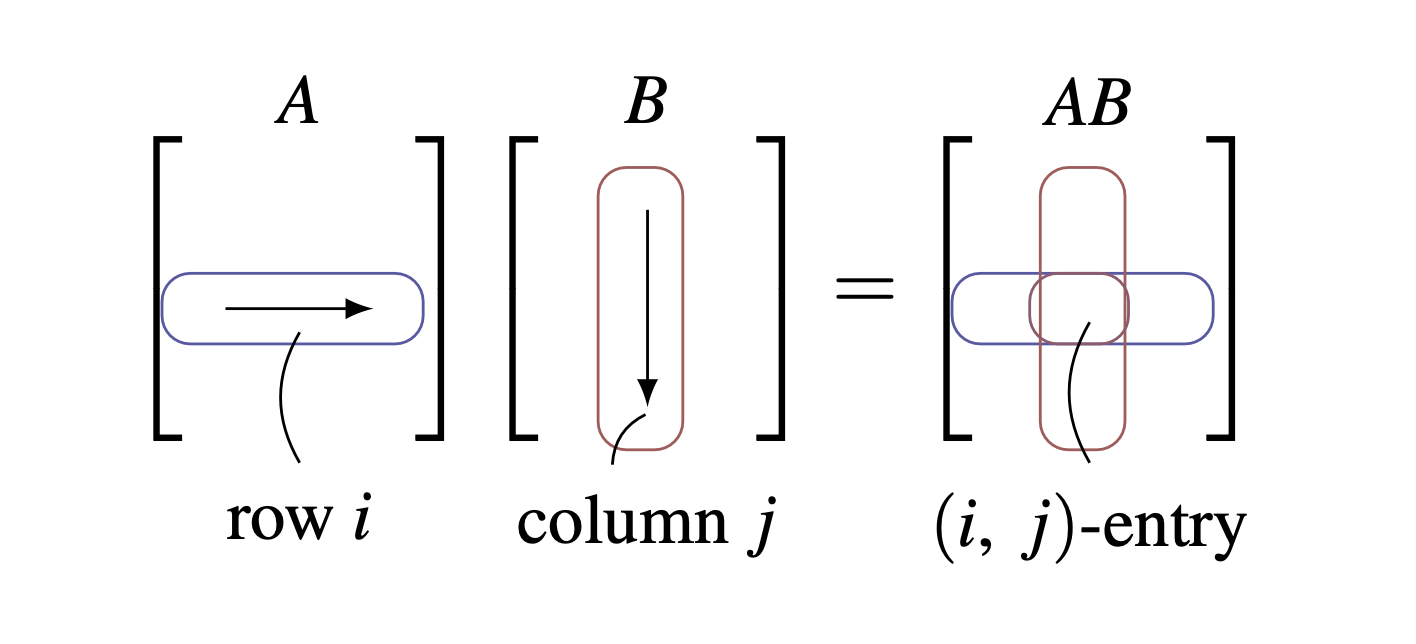
\includegraphics[width=4in]{AB-dotproduct}
	\caption{From Linear Algebra with Applications, Vretta-Lyryx}
\end{figure}


\question When is the product of two matrices $A$ and $B$ defined? What is the size of the product $AB$? 


\bigskip

\activity Let 
\[
A = \left[ \begin{array}{rrr}
-3 & -4 & 1 \\  
2 &  4 & 0 \\ 
1 & -4 & -5 \\
\end{array}\right] 
\text{ and } B = \left[ \begin{array}{rrr}
-1 & 2 & -4 \\ 
-4 & -3 & -1 \\ 
4 & 3 & 1
\end{array} \right].
\]

What is the $(2,3)$ entry of $AB$? 

\answer[2cm]{
	$\text{Row 2 } \cdot \text{ Column 3: }$ 
	
	$(2)(-4) + (4)(-1) + (0)(1) = -8 - 4 + 0 = -12$
}

\bigskip

\topic{Properties of Matrix Multiplication} Assume that $A,B,C$ are matrices of appropriate sizes. Then:
\begin{enumerate}[(a)]
	\item $A(BC)=\fillin{(AB)C}$, i.e. matrix multiplication is \fillin{associative}. 
	\item $(A+B)C=\fillin{AC + BC}$. 
	\item $C(A+B)=\fillin{CA + CB}$. 
	\item $A(rB)=\fillin{r(AB)}=\fillin{(rA)B}$. 
	\item $(AB)^T=\fillin{B^TA^T}$
	
\end{enumerate}



\emph{Proof of (d) (if time):}

\answer{
	Let $A$ be an $m \times n$ matrix and $B$ be an $n \times k$ matrix. Then:
	
	$A(rB) = A[rb_{ij}] = [\sum_{j=1}^n a_{ij} (rb_{jk})] = r[\sum_{j=1}^n a_{ij}b_{jk}] = r(AB)$
	
	Similarly,
	$(rA)B = [ra_{ij}][b_{jk}] = [\sum_{j=1}^n (r a_{ij}) b_{jk}] = r[\sum_{j=1}^n a_{ij}b_{jk}] = r(AB)$
}

\bigskip

\begin{framed}
\textit{Facts and Warnings about Matrix Multiplication}: Let $A$ be an $m \times p$ matrix and $B$ be a $p \times n$ matrix, so that their product $AB$ is defined and is a \fillin{$m \times n$} matrix. 
\begin{enumerate}
    \item The product $BA$ may not be defined! 
    \item If $BA$ is also defined, the size of $AB$ and $BA$ may be the same or different. 
    \item In the case where $AB$ and $BA$ are the same size, $AB$ and $BA$ may be equal or they may be different.
\end{enumerate}
\end{framed}


\activity Let 
$
A = \twobytwo{0}{-1}{-1}{5} 
\text{ and } 
B = \twobytwo{3}{3}{-4}{-3}.
$

Calculate and compare $AB$ and $BA$, if they are defined. 

\answer[5cm]{
	\[AB = \begin{bmatrix}
		4 & 3 \\
		-23 & -18
	\end{bmatrix}\]
	
	\[BA = \begin{bmatrix}
		-3 & 12 \\
		3 & -11
	\end{bmatrix}\]
	
	The products $AB$ and $BA$ exist but are not equal.
}


\activity Consider the following matrices:
\[A = \begin{bmatrix}1 & 2 & 3\\4 & 5 & 6\end{bmatrix}, \quad 
B = \begin{bmatrix}1 & 2\\3 & 4\\5 & 6\end{bmatrix}, \quad
C = \begin{bmatrix}1 & 2\\3 & 4\end{bmatrix}\]

For each of the following products, determine (i) whether the product is defined, and (ii) if defined, what is the size of the resulting matrix.

$AB$ and $BA$:

\answer[9cm]{
	For $AB$: Matrix $A$ is $2\times 3$ and matrix $B$ is $3\times 2$
	\begin{itemize}
		\item $AB$ is defined because the number of columns of $A$ (3) equals the number of rows of $B$ (3)
		\item The resulting matrix will be $2\times 2$
	\end{itemize}
	
	For $BA$: Matrix $B$ is $3\times 2$ and matrix $A$ is $2\times 3$
	\begin{itemize}
		\item $BA$ is defined because the number of columns of $B$ (2) equals the number of rows of $A$ (2)
		\item The resulting matrix will be $3\times 3$
	\end{itemize}
}

$BC$ and $CB$:

\answer[8cm]{
	For $BC$: Matrix $B$ is $3\times 2$ and matrix $C$ is $2\times 2$
	\begin{itemize}
		\item $BC$ is defined because the number of columns of $B$ (2) equals the number of rows of $C$ (2)
		\item The resulting matrix will be $3\times 2$
	\end{itemize}
	
	For $CB$: Matrix $C$ is $2\times 2$ and matrix $B$ is $3\times 2$
	\begin{itemize}
		\item $CB$ is not defined because the number of columns of $C$ (2) does not equal the number of rows of $B$ (3)
	\end{itemize}
}

\textit{Key property of identity matrices} If $A$ is any $\mbyn$ matrix, then 
\[
A I_n = A 
\text{ and }
I_m A = A.
\]

\bigskip

\topic{Matrix Powers} Using the definition of matrix multiplication, we can also define the powers of square matrices. Let $A$ be a square matrix. Then 
\[ 
A^2 = \fillin{A A}, \quad A^3 = \fillin{A A A}, \quad \text{etc.}
\]
We make the convention that 
\[
A^0 = \fillin{I} 
\]

If $p$ and $q$ are nonnegative integers, then 
\[
A^pA^q = \fillin{A^{p+q}}
\text{ and }
(A^p)^q = \fillin{A^{pq}}.
\]

\textit{Warning!} It is not necessarily the case that $(AB)^p = A^pB^p$. Why? 


\newpage



\sectiontitle{2.4}{Linear Transformations}

What makes a transformation a matrix transformation?


\definition A transformation $T:\mathbb{R}^n\to\mathbb{R}^m$ is a \fillin{linear transformation} if
\begin{enumerate}[(a)]
    \item $T(\bfx + \bfy) = \fillin{T(\bfx) + T(\bfy)}$ for every $\bfx, \bfy \in \mathbb{R}^n$.
    \item $T(c\bfx)=\fillin{c T(\bfx)}$ for every $\bfx \in \mathbb{R}^n$ and $c \in \bbR$.
    \end{enumerate}


\activity Using $\mathbb{R}=\mathbb{R}^1$, determine whether $T(x)=2x$ and $T(x)=x^2$ are linear transformations. Explain your reasoning.

\answer[6cm]{
	For $T(x)=2x$:
	\begin{align*}
		T(x+y) &= 2(x+y) = 2x + 2y = T(x) + T(y)\\
		T(cx) &= 2(cx) = c(2x) = cT(x)
	\end{align*}
	For $T(x)=x^2$:
	\begin{align*}
		T(x+y) &= (x+y)^2 = x^2 + 2xy + y^2 \neq x^2 + y^2 = T(x) + T(y)
	\end{align*}
}

\bigskip

\activity If $T$ is a linear transformation, what is...

$T(\mathbf{0})$?

\answer[1cm]{
	$T(\mathbf{0}) = T(0 \mathbf{0}) = 0 T(\mathbf{0})$, so $T(\mathbf{0}) = \mathbf{0}$
}

$T(-\mathbf{x})$?

\answer[1cm]{
	$T(-\mathbf{x}) = T((-1)\mathbf{x}) = (-1)T(\mathbf{x}) = -T(\mathbf{x})$
}


Recall: A vector $\bfy\in\mathbb{R}^n$ is a \fillin{linear combination} of vectors $\bfx_1, \bfx_2,\ldots \bfx_k$ if there are scalars $a_1, a_2, \ldots, a_k$ such that

$$\bfy=a_1\bfx_1+a_2\bfx_2+\cdots a_k\bfx_k.$$

\bigskip

\theorem If $T:\mathbb{R}^n\to\mathbb{R}^m$ is a linear transformation, then 

\bigskip

$T(a_1\bfx_1+a_2\bfx_2+\cdots a_k\bfx_k)= \fillin{a_1T(\mathbf{x}_1) + a_2T(\mathbf{x}_2) + \cdots + a_kT(\mathbf{x}_k)}$

\bigskip

\activity Suppose $T:\mathbb{R}^2\to\mathbb{R}^3$ is a linear transformation with $T\left(\begin{bmatrix} 1 \\ 2\end{bmatrix}\right)=\begin{bmatrix} -1 \\ 0 \\ 3\end{bmatrix}$, $T\left(\begin{bmatrix} -1 \\0\end{bmatrix}\right)=\begin{bmatrix} 4\\ 1 \\ 2\end{bmatrix}$. Find $T\left(\begin{bmatrix} 3 \\ 4\end{bmatrix}\right)$.

\bigskip

\answer[16cm]{
	Need to write $\begin{bmatrix} 3 \\ 4 \end{bmatrix}$ as a linear combination of $\begin{bmatrix} 1 \\ 2 \end{bmatrix}$ and $\begin{bmatrix} -1 \\ 0 \end{bmatrix}$.
	
	Let $a,b$ be scalars such that:
	$\begin{bmatrix} 3 \\ 4 \end{bmatrix} = a\begin{bmatrix} 1 \\ 2 \end{bmatrix} + b\begin{bmatrix} -1 \\ 0 \end{bmatrix}$
	This gives us the system:
	\begin{align*}
		a - b &= 3 \\
		2a &= 4
	\end{align*}
	From the second equation: $a = 2$
	Substituting into first equation: $2 - b = 3$, so $b = -1$
	
	Therefore: $\begin{bmatrix} 3 \\ 4 \end{bmatrix} = 2\begin{bmatrix} 1 \\ 2 \end{bmatrix} - \begin{bmatrix} -1 \\ 0 \end{bmatrix}$
	
	By linearity of $T$:
	\begin{align*}
		T\begin{bmatrix} 3 \\ 4 \end{bmatrix} &= 2\begin{bmatrix} -1 \\ 0 \\ 3 \end{bmatrix} - \begin{bmatrix} 4 \\ 1 \\ 2 \end{bmatrix}
		= \begin{bmatrix} -2 \\ 0 \\ 6 \end{bmatrix} - \begin{bmatrix} 4 \\ 1 \\ 2 \end{bmatrix}
		= \begin{bmatrix} -6 \\ -1 \\ 4 \end{bmatrix}
	\end{align*}
}

\bigskip

\theorem Let $T:\mathbb{R}^n\to\mathbb{R}^m$ be a transformation.

\begin{itemize}
    \item[1.] $T$ is a linear transformation if and only if it is a matrix transformation.
    \item[2.] In this case, $T=T_A$ is the matrix transformation induced by the unique matrix $A$, given in terms of its columns by 

    $$A=\begin{bmatrix} T(\mathbf{e}_1) & T(\mathbf{e}_2) & \cdots & T(\mathbf{e}_n) \end{bmatrix},$$
    where $\mathbf{e}_1,\mathbf{e}_2, \ldots \mathbf{e}_n$ are the standard basis vectors of $\mathbb{R}^n$.
\end{itemize}
\emph{Proof (if time):}

\answer[12cm]{
	First show that if $T$ is a matrix transformation, then it is linear:
	If $T = T_A$ for some matrix $A$, then:
	$T(\mathbf{x} + \mathbf{y}) = A(\mathbf{x} + \mathbf{y}) = A\mathbf{x} + A\mathbf{y} = T(\mathbf{x}) + T(\mathbf{y})$, 
	$T(c\mathbf{x}) = A(c\mathbf{x}) = cA\mathbf{x} = cT(\mathbf{x})$
	
	Now show that if $T$ is linear, then it is a matrix transformation:
	Let $A = \begin{bmatrix} T(\mathbf{e}_1) & T(\mathbf{e}_2) & \cdots & T(\mathbf{e}_n) \end{bmatrix}$.
	For any $\mathbf{x} = \begin{bmatrix} x_1 \\ x_2 \\ \vdots \\ x_n \end{bmatrix}$, we can write:
	$\mathbf{x} = x_1\mathbf{e}_1 + x_2\mathbf{e}_2 + \cdots + x_n\mathbf{e}_n$.
	
	Then by linearity:
	$T(\mathbf{x}) = T(x_1\mathbf{e}_1 + x_2\mathbf{e}_2 + \cdots + x_n\mathbf{e}_n)$
	$= x_1T(\mathbf{e}_1) + x_2T(\mathbf{e}_2) + \cdots + x_nT(\mathbf{e}_n)$
	$= A\mathbf{x}$.
	
	Therefore $T = T_A$ is a matrix transformation.
	
	For uniqueness, suppose $T = T_B$ for some other matrix $B$. Then:
	$A\mathbf{e}_i = T(\mathbf{e}_i) = B\mathbf{e}_i$ for all $i$.
	Therefore the columns of $A$ and $B$ are identical, so $A = B$.
}

\bigskip

\corollary If $T:\mathbb{R}^k\to\mathbb{R}^n$, and $S:\mathbb{R}^n\to\mathbb{R}^m$ are linear transformations, then $S\circ T$ is a linear transformation.

%\bigskip
\newpage

\activity Consider the linear transformation $T:\mathbb{R}^2\to\mathbb{R}^2$ defined by 
$T\left(\begin{bmatrix} x \\ y \end{bmatrix}\right)=\begin{bmatrix} 3x + \frac{3}{2}y \\ x + 2y \end{bmatrix}$. 
Find the matrix $A$ such that $T = T_A$.

\bigskip

\answer[8cm]{
	To find the matrix $A$, we need to find the images of the standard basis vectors under $T$:
	
	$T(\mathbf{e}_1) = T\left(\begin{bmatrix} 1 \\ 0 \end{bmatrix}\right) = \begin{bmatrix} 3(1) + \frac{3}{2}(0) \\ 1(1) + 2(0) \end{bmatrix} = \begin{bmatrix} 3 \\ 1 \end{bmatrix}$
	
	$T(\mathbf{e}_2) = T\left(\begin{bmatrix} 0 \\ 1 \end{bmatrix}\right) = \begin{bmatrix} 3(0) + \frac{3}{2}(1) \\ 1(0) + 2(1) \end{bmatrix} = \begin{bmatrix} \frac{3}{2} \\ 2 \end{bmatrix}$
	
	Therefore, by the theorem, the matrix is:
	
	$A = \begin{bmatrix} T(\mathbf{e}_1) & T(\mathbf{e}_2) \end{bmatrix} = \begin{bmatrix} 3 & \frac{3}{2} \\ 1 & 2 \end{bmatrix}$
}

\bigskip

The following figure provides a visualization 
of this transformation.
\begin{figure}[h]
	\centering
	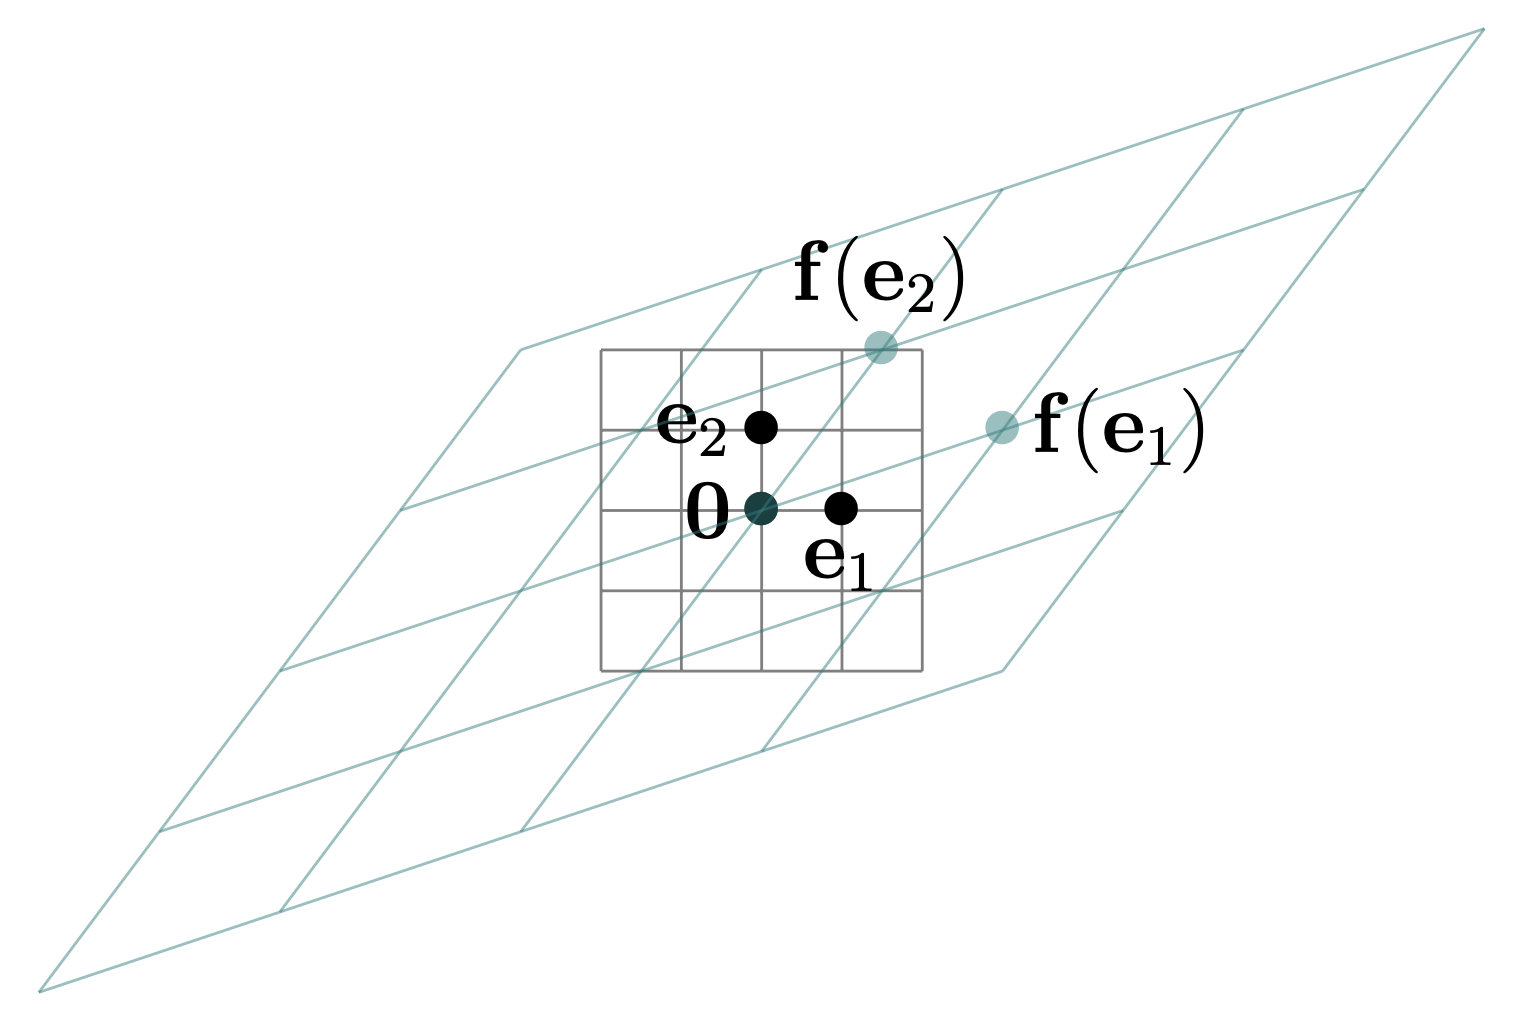
\includegraphics[width=0.66\textwidth]{math-51-fig-13-4-1.png}
	\caption{The distorted (aqua) grid obtained by applying the linear transformation $\mathbf{f}(\mathbf{x}) = T(\mathbf{x})$ to a (gray) square grid. From: Stanford's MATH 51 textbook}
	\label{fig:linear-transformation-grid}
\end{figure}

%\bigskip
\newpage

\activity Define $T:\mathbb{R}^2\to\mathbb{R}^3$ by $T\left(\begin{bmatrix} x_1 \\ x_2 \end{bmatrix}\right)=\begin{bmatrix} x_1 +x_2 \\ x_1 \\ 3x_2 \end{bmatrix}$. Show $T$ is a linear transformation.


\answer[8cm]{
	$T(\mathbf{x} + \mathbf{y}) = \begin{bmatrix} (x_1+y_1)+(x_2+y_2) \\ x_1+y_1 \\ 3(x_2+y_2) \end{bmatrix} = \begin{bmatrix} x_1+x_2 \\ x_1 \\ 3x_2 \end{bmatrix} + \begin{bmatrix} y_1+y_2 \\ y_1 \\ 3y_2 \end{bmatrix} = T(\mathbf{x}) + T(\mathbf{y})$
	
	$T(c\mathbf{x}) = \begin{bmatrix} cx_1+cx_2 \\ cx_1 \\ 3cx_2 \end{bmatrix} = c\begin{bmatrix} x_1+x_2 \\ x_1 \\ 3x_2 \end{bmatrix} = cT(\mathbf{x})$
}


Find $A$, where $T=T_A$.

\answer[3cm]{
	$A = \begin{bmatrix} T(\mathbf{e}_1) & T(\mathbf{e}_2) \end{bmatrix} = \begin{bmatrix} 1 & 1 \\ 1 & 0 \\ 0 & 3 \end{bmatrix}$
}

\bigskip

Is there an $\mathbf{x}$ in $\mathbb{R}^2$ with $T(\mathbf{x})=\begin{bmatrix} 4 \\ -1 \\ 6\end{bmatrix}?$

\bigskip

\answer[6cm]{
	We need to solve $A\mathbf{x} = \begin{bmatrix} 4 \\ -1 \\ 6 \end{bmatrix}$
	This gives the system:
	$x_1 + x_2 = 4$,
	$x_1 = -1$,
	$3x_2 = 6$
	
	From third equation: $x_2 = 2$.
	From second equation: $x_1 = -1$.
	This does not satisfy first equation: $-1 + 2 = 1 \neq 4$
	
	Therefore, there is no such $\mathbf{x}$.
}


%\newpage



\sectiontitle{2.5}{Matrix Inverses}


\definition An $\nbyn$ matrix $A$ is called \fillin{nonsingular}, or \fillin{invertible}, if there exists an $\nbyn$ matrix $B$ such that \fillin{$AB = BA = I_n$}. Such a $B$ is called the \fillin{inverse} of $A$. If no such $B$ exists, $A$ is called \fillin{singular} or \fillin{noninvertible}. 

\bigskip 

\textit{Idea}: The inverse of a matrix mimics the reciprocal of a real number. 

\bigskip

\activity Let $A = \twobytwo{1}{3}{1}{4}$ and $B = \twobytwo{4}{-3}{-1}{1}$. Compute both $AB$ and $BA$, and make a conclusion using the language of inverses. 

\answer[3cm]{
	\[
	AB = \left[\begin{array}{cc}
		1 & 0 \\
		0 & 1
	\end{array}\right] = I_2
	\quad\text{and}\quad
	BA = \left[\begin{array}{cc}
		1 & 0 \\
		0 & 1
	\end{array}\right] = I_2\]
	
	$\text{Therefore, } B \text{ is the inverse of } A.$
}

\bigskip 

\textit{Fact:} The inverse of a matrix, if it exists, is unique. Therefore, we can write \fillin{$A^{-1}$} for the inverse of $A$. 


\bigskip

\textit{Fact:} If $AB = I_n$, then $BA = I_n$. 


%\bigskip 
\newpage

\activity Does $A=\begin{bmatrix} 2 & 1 \\ 0 & 0 \end{bmatrix}$ have an inverse?

\answer[14cm]{
	Let's suppose $A$ had an inverse $B = \begin{bmatrix} x & y \\ z & w \end{bmatrix}$. Then:
	\begin{align*}
		AB &= I_2\\[5pt]
		\begin{bmatrix} 2 & 1 \\ 0 & 0 \end{bmatrix}\begin{bmatrix} x & y \\ z & w \end{bmatrix} &= \begin{bmatrix} 1 & 0 \\ 0 & 1 \end{bmatrix}
	\end{align*}
	
	This gives us the system of equations:
	\begin{align*}
		2x + z &= 1\\
		2y + w &= 0\\
		0x + 0z &= 0\\
		0y + 0w &= 1
	\end{align*}
	
	The last equation states that $0 = 1$, which is impossible.
	
	Therefore, $A$ cannot have an inverse. This means $A$ is singular.
}


\textit{Theorem:} If both $A$ and $B$ are nonsingular $\nbyn$ matrices, then the matrix $AB$ is \fillin{nonsingular} and its inverse is $(AB)\inv = $\fillin{$B^{-1} A^{-1}$}. 

\medskip 

\textit{Proof:}

\answer[3cm]{
	First, $(AB)(B^{-1}A^{-1}) = A(BB^{-1})A^{-1} = A I_n A^{-1} = AA^{-1} = I_n$
	
	Similarly, $(B^{-1}A^{-1})(AB) = B^{-1}(A^{-1}A)B = B^{-1} I_n B = B^{-1}B = I_n$
}

%\bigskip
\newpage

Follow up facts:
\begin{itemize}
	\item If $A_1, A_2,\ldots, A_k$ are $n\times n$ invertible/nonsingular matrices, then $A_1A_2\cdots A_k$ is invertible/nonsingular and $(A_1A_2\cdots A_k)^{-1}=\fillin{A_k^{-1}\cdots A_2^{-1} A_1^{-1}}$
	\item If $A$ is invertible/nonsingular, then $A^{-1}$ is invertible/nonsingular and $(A^{-1})^{-1}=\fillin{A}$.
	\item If $A$ is invertible/nonsingular, then $A^T$ is invertible/nonsingular and $(A^{-1})^T=\fillin{(A^T)^{-1}}$. 
\end{itemize}


\theorem (Inverse of $2\times 2$ matrix) The $2\times 2$ matrix $$A=\begin{bmatrix}
	a & b \\ c & d
\end{bmatrix}$$
is invertible if and only if $ad-bc\neq 0$, in which case

$$A^{-1}=\dfrac{1}{ad-bc}\begin{bmatrix}
	d & -b \\ -c & a
\end{bmatrix}$$

We'll learn how to compute inverses for bigger matrices soon.

\activity Find the inverse of each matrix, if possible.

$$A=\begin{bmatrix}
	-2 & -3 \\ 4 & 6
\end{bmatrix},\; B=\begin{bmatrix}
	1 & 6 \\ 2 & 3
\end{bmatrix} $$

\answer{
	For $A$: $\det(A) = (-2)(6) - (-3)(4) = -12 - (-12) = 0$, so $A$ is not invertible.
	
	For $B$: $\det(B) = (1)(3) - (6)(2) = 3 - 12 = -9 \neq 0$, so
	$B^{-1} = \frac{1}{-9}\twobytwo{3}{-6}{-2}{1} = \twobytwo{-1/3}{2/3}{2/9}{-1/9}$
}

%\bigskip
\newpage

\topic{Linear Systems and Inverses} 

If $A$ is an $\nbyn$ matrix, then the linear system $A\bfx = \bfb$ is a system of \fillin{$n$} equations in \fillin{$n$} unknowns. Suppose $A$ is nonsingular. How can we use $\Ainv$ to solve the system $A\bfx = \bfb$? 

\answer[9cm]{
	Multiply both sides of $A\bfx = \bfb$ by $\Ainv$ on the left:
	\begin{align*}
		A\bfx &= \bfb\\
		\Ainv(A\bfx) &= \Ainv\bfb\\
		(\Ainv A)\bfx &= \Ainv\bfb\\
		I_n\bfx &= \Ainv\bfb\\
		\bfx &= \Ainv\bfb
	\end{align*}
	
	Therefore, when $A$ is nonsingular, $\bfx = \Ainv\bfb$ is the solution to $A\bfx = \bfb$.
}

\textit{Consequences}: 
\begin{itemize}
	\item When $\Ainv$ exists, then $A\bfx = \bfb$ has a \fillin{unique} solution. 
	\item If $A$ is invertible/nonsingular, then the ONLY solution to the homogeneous system \fillin{$A\bfx = \bfzero$} is $\bfx =\fillin{\bfzero}$. 
\end{itemize}

%\bigskip
\newpage

\activity Use the inverse of $A$ to solve the linear systems $A\bfx = \bfb$, $A\bfx = {\bfc}$, and $A\bfx = \bfzero$, where $A$, $\bfb$, and ${\bfc}$ are given below. 
\[
A = \twobytwo{1}{2}{3}{4}, 
\quad 
\Ainv = \twobytwo{-2}{1}{\frac{3}{2}}{-\frac{1}{2}}, 
\quad
\bfb = \colvec{4 \\ 2},
\ \text{ and } \ 
{\bfc} = \colvec{3 \\ 2}.
\]

\answer[6cm]{
	For $A\bfx = \bfb$: $\bfx = A^{-1}\bfb = \twobytwo{-2}{1}{\frac{3}{2}}{-\frac{1}{2}}\colvec{4 \\ 2} = \colvec{-6 \\ 5}$
	
	For $A\bfx = \bfc$: $\bfx = A^{-1}\bfc = \twobytwo{-2}{1}{\frac{3}{2}}{-\frac{1}{2}}\colvec{3 \\ 2} = \colvec{-4 \\ \frac{7}{2}}$
	
	For $A\bfx = \bfzero$: $\bfx = A^{-1}\bfzero = \colvec{0 \\ 0}$
}

%\bigskip
% \newpage

\topic{Algorithm for Calculating Inverses}

For a given $n\times n$ matrix $A$, if we are looking for an inverse for $A$ (call this matrix $X$), we must have $AX=I_n$. We are solving $n$ linear systems simultaneously:

\answer{
	$A\begin{bmatrix} x_{11} \\ x_{21} \\ \vdots \\ x_{n1} \end{bmatrix} = \begin{bmatrix} 1 \\ 0 \\ \vdots \\ 0 \end{bmatrix},\ 
	A\begin{bmatrix} x_{12} \\ x_{22} \\ \vdots \\ x_{n2} \end{bmatrix} = \begin{bmatrix} 0 \\ 1 \\ \vdots \\ 0 \end{bmatrix},\ 
	\cdots,\ 
	A\begin{bmatrix} x_{1n} \\ x_{2n} \\ \vdots \\ x_{nn} \end{bmatrix} = \begin{bmatrix} 0 \\ 0 \\ \vdots \\ 1 \end{bmatrix}$
}

Since, to solve each system, we wish to reduce the matrix $A$ down to its RREF each time, we can combine all the systems into one big augmented matrix:

\answer{
	$[A \mid I_n] = \left[\begin{array}{rrrr|rrrr} 
		a_{11} & a_{12} & \cdots & a_{1n} & 1 & 0 & \cdots & 0 \\
		a_{21} & a_{22} & \cdots & a_{2n} & 0 & 1 & \cdots & 0 \\
		\vdots & \vdots & \ddots & \vdots & \vdots & \vdots & \ddots & \vdots \\
		a_{n1} & a_{n2} & \cdots & a_{nn} & 0 & 0 & \cdots & 1
	\end{array}\right]$
}

% Keep the algorithm heading with its steps on the next worksheet page.
\newpage
\begin{framed}\textbf{Algorithm for computing $A^{-1}$}
	
	\begin{itemize}
		\item Set up the augmented matrix $[A \dashline I_n]$.
		\item  Apply elementary row operations to $[A \dashline I_n]$ to reduce it to $[I_n \dashline \Ainv]$.
	\end{itemize}
	
	If $A$ is an $n\times n$ matrix, either $A$ can be reduced to $I_n$ by elementary row operations or it cannot. In
	the first case, the algorithm produces $A^{-1}$; in the second case, $A^{-1}$  does not exist.
\end{framed}

\bigskip
%\newpage

\activity Find $\Ainv$ where $A = \barray{rrr}{1 & 1 & 4 \\ 2 & 3 & 2 \\ 0 & 0 & 1}$. 

\answer[14cm]{
	$[A \dashline I_3] = \barray{rrr|rrr}{1 & 1 & 4 & 1 & 0 & 0 \\ 2 & 3 & 2 & 0 & 1 & 0 \\ 0 & 0 & 1 & 0 & 0 & 1}$
	
	$R_2 \to R_2 - 2R_1$:
	$\barray{rrr|rrr}{1 & 1 & 4 & 1 & 0 & 0 \\ 0 & 1 & -6 & -2 & 1 & 0 \\ 0 & 0 & 1 & 0 & 0 & 1}$
	
	$R_1 \to R_1 - R_2$:
	$\barray{rrr|rrr}{1 & 0 & 10 & 3 & -1 & 0 \\ 0 & 1 & -6 & -2 & 1 & 0 \\ 0 & 0 & 1 & 0 & 0 & 1}$
	
	$R_1 \to R_1 - 10R_3, R_2 \to R_2 + 6R_3$:
	$\barray{rrr|rrr}{1 & 0 & 0 & 3 & -1 & -10 \\ 0 & 1 & 0 & -2 & 1 & 6 \\ 0 & 0 & 1 & 0 & 0 & 1}$
	
	Therefore:
	$A^{-1} = \barray{rrr}{3 & -1 & -10 \\ -2 & 1 & 6 \\ 0 & 0 & 1}$
}


%\bigskip
\newpage


Below is a useful compilation of facts and theorems, some of which we've discussed in class. You can find the remainder of the proofs in your textbook. 

\begin{framed}\textbf{Box Of Facts/Invertibility Criteria}
	
	Let $A$ be an $\nbyn$ matrix. The following are equivalent: 
	\begin{enumerate}
		\item $A$ is nonsingular. 
		\item $A\bfx = \bfzero$ has only the trivial solution. 
		\item $A$ is row equivalent to $I_n$. 
		\item The linear system $A\bfx = \bfb$ has a unique solution for every $n \times 1$ matrix $\bfb$. 
		\item $\rank(A)=n$.
	\end{enumerate}
\end{framed}

\bigskip

\topic{Inverses of Matrix Transformations}

Let $T=T_A:\mathbb{R}^n\to\mathbb{R}^n$ be a matrix transformation induced by the $n\times n$ matrix $A$. What does invertibility imply about the geometry of the transformation $T_A$?

Consider $T'=T_{A^{-1}}$. What happens when we compose them?

\bigskip

$T\circ T'(\mathbf{x})=\shortanswer{T_A(T_{A^{-1}}(\mathbf{x})) = T_A(A^{-1}\mathbf{x}) = A(A^{-1}\mathbf{x}) = (AA^{-1})\mathbf{x} = I_n\mathbf{x} = \mathbf{x}}$

\bigskip

$T'\circ T(\mathbf{x})=\shortanswer{T_{A^{-1}}(T_A(\mathbf{x})) = T_{A^{-1}}(A\mathbf{x}) = A^{-1}(A\mathbf{x}) = (A^{-1}A)\mathbf{x} = I_n\mathbf{x} = \mathbf{x}}$

\bigskip

\definition  Given a matrix transformation $T:\mathbb{R}^n\to\mathbb{R}^n$, if there exists a transformation $S:\mathbb{R}^n\to\mathbb{R}^n$ such that $S(T(\mathbf{x}))=\fillin{T(S(\mathbf{x}))}=\fillin{\mathbf{x}}$ for all $\mathbf{x}\in \mathbb{R}^n$, we say that $T$ has an inverse.

\bigskip

\theorem Let $T:\mathbb{R}^n\to\mathbb{R}^n$ denote the matrix transformation induced by an $n\times n$ matrix $A$. Then
$A$ is invertible if and only if $T$ has an inverse.
In this case, $T$ has exactly one inverse (which we denote as $T^{-1}$), and $T^{-1} : \mathbb{R}^n\to\mathbb{R}^n$ is the
transformation induced by the matrix $A^{-1}$. In other words
$$(T_A)^{-1} = T_{A^{-1}}$$

$T$ and $T^{-1}$ ``reverse'' or ``undo'' the action of each other.

%\bigskip
\newpage

\activity Consider $T:\mathbb{R}^2\to\mathbb{R}^2$ given by reflection across the $x$-axis. Find the matrix representing this transformation, and find the inverse.


\answer{
	T is given by matrix $A = \twobytwo{1}{0}{0}{-1}$
	
	Since $A^2 = I_2$, $A$ is its own inverse, so $T^{-1} = T$
}

\activity Consider $P:\mathbb{R}^2\to\mathbb{R}^2$ by $P\left(\begin{bmatrix} a_1 \\ a_2\end{bmatrix}\right)=\begin{bmatrix} a_1 \\ 0\end{bmatrix}$. 

Is this a matrix transformation?


\answer[5cm]{
	Yes, $P$ is a matrix transformation. It can be represented by the matrix 
	$A = \begin{bmatrix} 1 & 0 \\ 0 & 0 \end{bmatrix}$
	
	To verify:
	$P\left(\begin{bmatrix} a_1 \\ a_2\end{bmatrix}\right) = \begin{bmatrix} 1 & 0 \\ 0 & 0 \end{bmatrix}\begin{bmatrix} a_1 \\ a_2\end{bmatrix} = \begin{bmatrix} a_1 \\ 0\end{bmatrix}$
}


Is this invertible?

\answer[2cm]{
	No, $P$ is not invertible. Note that $\det(A) = 0$, so $A$ is not invertible.
}


\end{document}

